\documentclass[a4paper,11pt]{report}
\usepackage[T1]{fontenc}
\usepackage[utf8]{inputenc}
\usepackage{lmodern}
\usepackage[spanish]{babel}
\usepackage{textcomp}
\usepackage{amsmath}
\usepackage{amsfonts}
\usepackage[framed,numbered,autolinebreaks]{mcode}
\usepackage{amssymb}
\usepackage{graphicx}
\usepackage{caption}
\usepackage{subcaption}
\usepackage{fancyhdr}
\usepackage{float}
\usepackage{color}
\usepackage[left=2cm,right=2cm,top=2cm,bottom=2cm]{geometry}

\title{Serie 2}
\author{Alamilla Ortiz Cesar Alejandro\\Cabrera López Óscar Emilio\\Castillo Cruz Heriberto\\Cuevas Mondragón Ricardo\\Equipo 9}

\pagestyle{fancy}
\fancyhf{}
\lhead[]{}
\chead[]{}
\rfoot{\thepage}
\lfoot[]{}
\cfoot[]{}

\renewcommand\headrule
{{\color[RGB]{98,36,35}%
    \hrule height 2pt
    width\headwidth
    \vspace{1.3pt}%
    \hrule height 1pt
    width\headwidth
  }}
  \addto\captionsspanish{\def\tablename{Tabla}}%imprime Tabla en lugar de Cuadro
  %%
  \spanishdecimal{.}


\begin{document}
\thispagestyle{fancy}
\maketitle
\tableofcontents
\newpage
\setcounter{chapter}{1}

\section{Ejercicio 1}
Considere el sistema de primer orden cuyo modelo corresponde a una ecuación diferencial de primer orden
\begin{equation}
  \frac{dy\left(t\right)}{dt} + 3y\left(t\right) = x\left(t\right)
  \label{mod_sist}
\end{equation}
Determine:
\begin{enumerate}
  \item[a)] La respuesta $y\left(t\right)$ a la entrada escalón $u\left(t\right)$,mediante algún método en el dominio del tiempo y presente la gráfica correspondiente.\newline
    Resolviendo la ecuación homogénea:
    \begin{equation}
      \begin{split}
       \left(D + 3\right)y\left(t\right) & = 0\\
        P\left(\lambda\right) = \lambda + 3 & = 0\\
        \quad \lambda & = -3\\
        y_h\left(t\right) & = c_{1}e^{-3t}
      \end{split}
      \label{sol_h}
    \end{equation}
    Dado que el escalón toma un valor constante para cualquier $t >  0$ la solución particular a la ecuación diferencial tendrá la forma de
    \[ y_{p}\left(t\right) = A\quad;\quad A \in \mathbb{R} \]
    Por lo tanto
    \[
      \begin{split}
      y_p\left(t\right) & = A\\
      \dot y_p\left(t\right) & = 0\\
      \end{split}
    \]
    Sustituyendo $y_p\left(t\right)$ en (\ref{mod_sist})
    \[
      \begin{split}
        3A & = u\left(t\right)\\
        A & = \frac{1}{3}u\left(t\right)
      \end{split}
    \]
    Nuestra solución general es entonces: 
    \[
      y_g\left(t\right) = \left(c_1e^{-3t} + \frac{1}{3}\right)u\left(t\right)
    \]
    Entonces, si consideramos que $y_g\left(0\right) = 0$ tenemos que
    \[
      \begin{split}
        c_1 + \frac{1}{3} & = 0 \\
        c_1 & = -\frac{1}{3}
      \end{split}
    \]
    Finalmente 
    \[
      y_g\left(t\right) = \left(-\frac{1}{3}e^{-3t} + \frac{1}{3}\right)u\left(t\right)
      \label{sol_g}
    \]
    Código en Matlab:
    \lstinputlisting{./Ejercicio1/resp_escalon.m}
    \begin{figure}[H]
      \begin{center}
        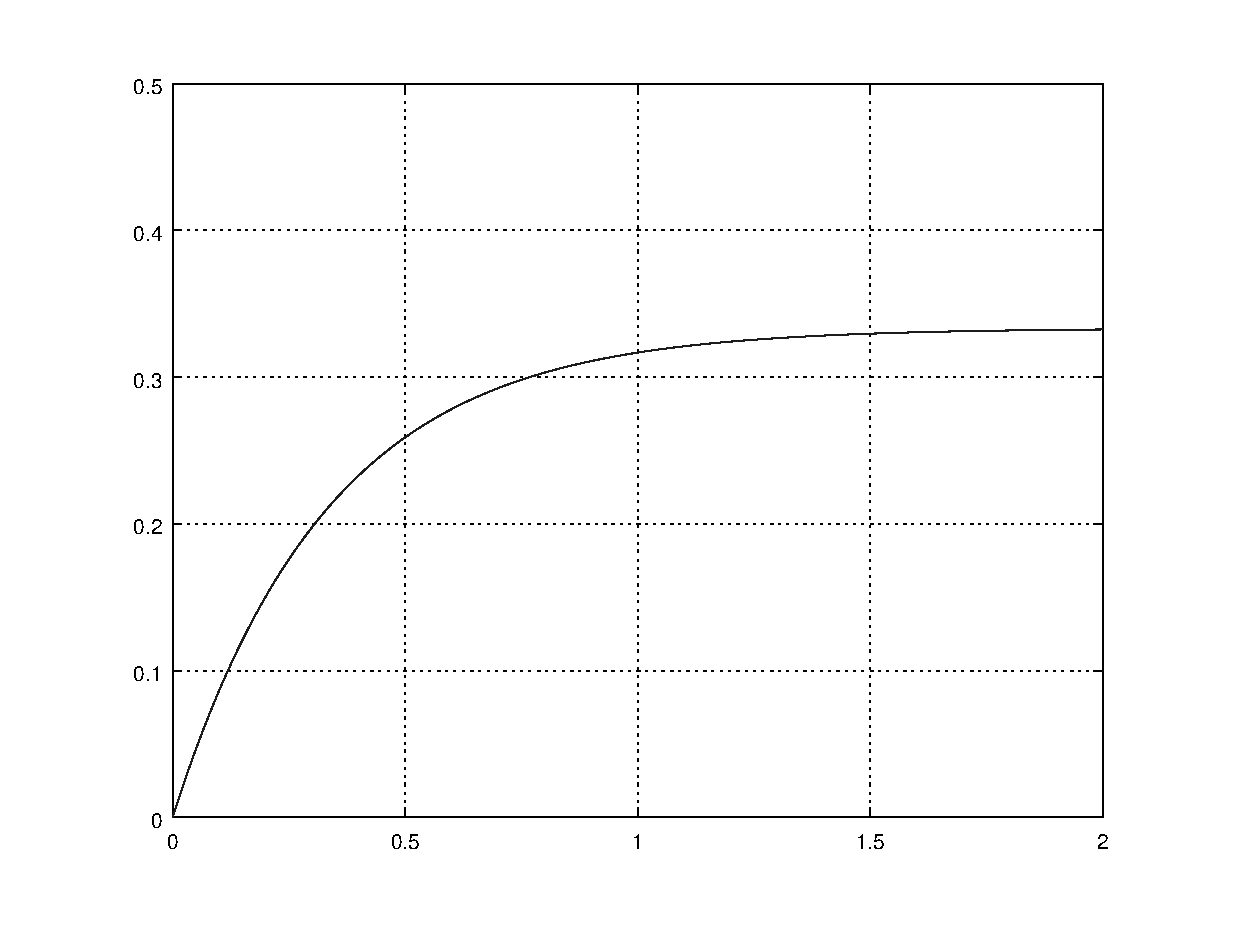
\includegraphics[width=0.55\textwidth]{./Ejercicio1/resp_escalon}
        \caption{Respuesta al escalón}
      \end{center}
    \end{figure}
  \item[b)] Obtenga la constante de tiempo $\tau$ e identifíquela en la gráfica.\newline
    Si factorizamos la respuesta al escalón, es más fácil identificar la constante de tiempo $\tau$ y la amplitud $M$
    \[ y\left(t\right) = M\left(1 - e^{-\frac{t}{\tau}}\right)u\left(t\right) \]
    \[ y\left(t\right) = \frac{1}{3}\left(1 - e^{-3t}\right)u\left(t\right) \]
    \[ \therefore \qquad \tau = \frac{1}{3} \quad ; \quad M = \frac{1}{3} \]
    Código en Matlab:
    \lstinputlisting{./Ejercicio1/resp_escalon_tau.m}
    \begin{figure}[H]
      \begin{center}
        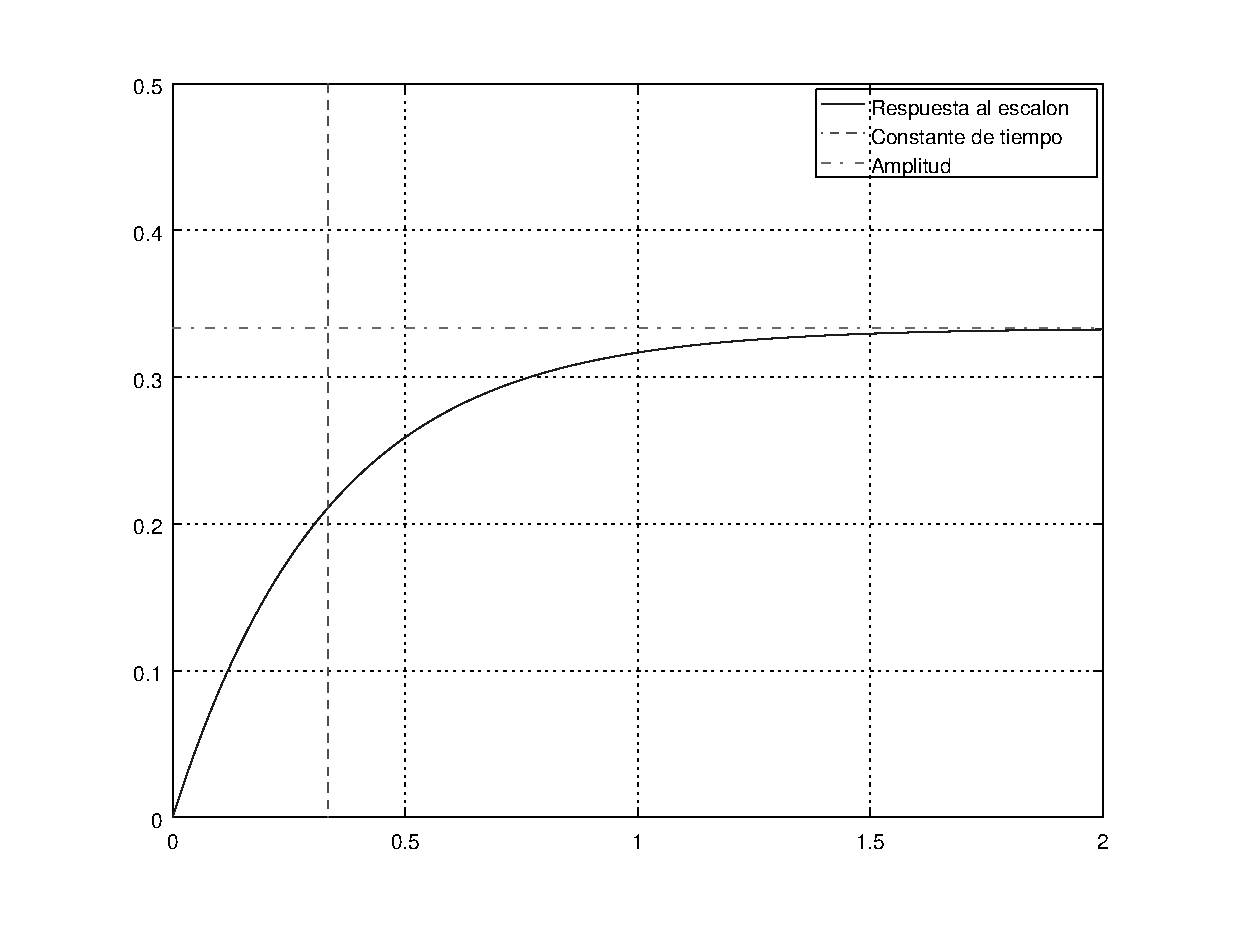
\includegraphics[width=0.6\textwidth]{./Ejercicio1/resp_escalon_tau}
        \caption{Constante de tiempo}
      \end{center}
    \end{figure}
  \item[c)] La respuesta $y_1\left(t\right)$ a la entrada $x_1\left(t\right)$ mediante algún método en el dominio del tiempo.
    \[ x_1\left(t\right) = r\left(t\right) \]
    Como la ecuación (\ref{sol_h}) aún es una solución válida debemos obtener solamente la solución particular del la ecuación diferencial que describe al sistema.\\
    Siguiendo un razonamiento similar al del inciso a, si recordamos la definición de la función rampa, veremos que la  solución particular tiene la forma de
    \[ y_p\left(t\right) = At + B \]
    ya  que:
    \[ r\left(t\right) = \;\left\{\begin{array}{lc}
                        t & t\geq0 \\
                        0 & t < 0 \\ 
                      \end{array}\right.
    \]
    Entonces:
    \[
      \begin{split}
      y_p\left(t\right) & = At + B\\
      \dot y_p\left(t\right) & = A\\
      \end{split}
    \]
    Sustituyendo en (\ref{mod_sist})
    \[
      \begin{split}
        A + 3At + 3B & = t\\
        3A & = 1\\
        A + 3B & = 0\\
        A = \frac{1}{3} & \quad B = -\frac{1}{9}
      \end{split}
    \]
    La solución general queda como:
    \[ y_g\left(t\right) = c_1e^{-3t} + \frac{1}{3}t - \frac{1}{9} \]
    Aplicando condiciones iniciales nulas:
    \[
      \begin{split}
        c_1 - \frac{1}{9} & = 0 \\
        c_1 & = \frac{1}{9}
      \end{split}
    \]
    Por lo que la respuesta del sistema a una entrada rampa es:
    \[ y_g\left(t\right) = \left( \frac{1}{9}e^{-3t} + \frac{1}{3}t - \frac{1}{9} \right)u\left(t\right) \]
  \item[d)] Obtenga la función de transferencia $H\left(s\right)$ del sistema
    \[
      \begin{split}
        \mathcal{L}\left\{ \frac{dy\left(t\right)}{dt} + 3y\left(t\right) = x\left(t\right) \right\} & = sY\left(s\right) + 3Y\left(s\right) = X\left(s\right)\\
        H\left(s\right) = \frac{Y\left(s\right)}{X\left(s\right)}& = \frac{1}{s + 3}
      \end{split}
    \]
  \item[e)] A partir de $H\left(s\right)$ determine la respuesta $y_1\left(t\right)$ a la entrada $x_1\left(t\right)$.
    \[ 
      \begin{split}
        Y\left(s\right) &= H\left(s\right)X\left(s\right)\\
        &= \frac{1}{s^2 \left(s + 3\right)} = \frac{A}{s} + \frac{B}{s^2} + \frac{C}{\left(s + 3\right)}\\
        A = -\frac{1}{9} \quad ; \quad  B = \frac{1}{3} \quad ; \quad C = \frac{1}{9}
      \end{split}
    \]
    Antitransformando tenemos:
    \[
      \mathcal{L}^{-1} \left\{ \frac{-\frac{1}{9}}{s} + \frac{\frac{1}{3}}{s^2} + \frac{\frac{1}{9}}{\left(s + 3\right)} \right\} = \left( - \frac{1}{9} + \frac{1}{3}t + \frac{1}{9}e^{-3t} \right) u\left(t\right)
    \]
    \newpage
    \item[f)] Obtenga las gráficas de $x_1\left(t\right)$ y de $y_1\left(t\right)$.\\
    Código en Matlab:
    \lstinputlisting{./Ejercicio1/resp_rampa.m}
    \begin{figure}[H]
      \begin{center}
        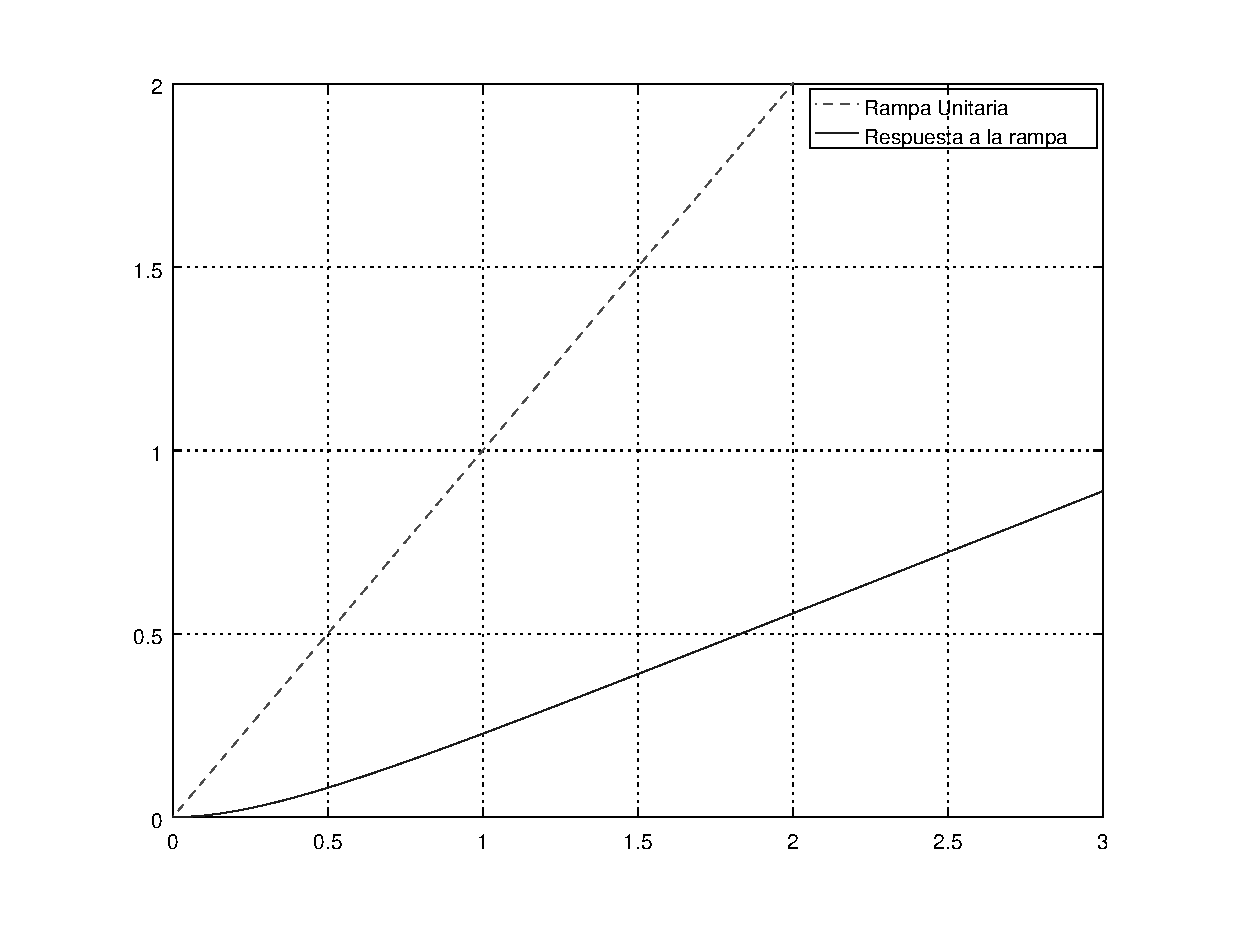
\includegraphics[width=0.6\textwidth]{./Ejercicio1/resp_rampa}
        \caption{Respuesta del sistema a la entrada de una señal rampa}
      \end{center}
    \end{figure}
\end{enumerate}

\section{Ejercicio 2}
Un modelo de sistema de 3° orden está definido mediante la ecuación diferencial indicada.
\[ \frac{d^3y\left(t\right)}{dt^3} +6\frac{d^2y\left(t\right)}{dt^2} + 11\frac{dy\left(t\right)}{dt} 6y\left(t\right) = \frac{1}{2}x\left(t\right) \]
La respuesta del sistema se compone de dos términos, la respuesta de estado cero y la respuesta de entrada
cero, las cuales a su vez pueden contener respuestas transitoria y/o permanente.
  \[ y\left(t\right) = y_{ZS}\left(t\right) + y_{ZI}\left(t\right) \]
Determine las respuestas indicadas, especificando en cada caso el tipo que corresponde de acuerdo con la
ecuación (1.4).
\begin{enumerate}
  \item[a)] La función de transferencia $H\left(s\right)$.
    \[ \mathcal{L}^{-1} \left\{ \frac{d^3y\left(t\right)}{dt^3} +6\frac{d^2y\left(t\right)}{dt^2} + 11\frac{dy\left(t\right)}{dt} 6y\left(t\right) = \frac{1}{2}x\left(t\right) \right\}  = \]
    \[ s^3Y\left(s\right) - s^2y\left(0\right) - sy'\left(0\right) - y''\left(0\right)  + 6\left( s^2Y\left(s\right) - sy\left(0\right) - y'\left(0\right) \right) + 11\left( sY\left(s\right) - y\left(0\right) \right) + 6Y\left(s\right) = \frac{1}{2}X\left(s\right)\]
    \[ s^3Y\left(s\right) + 6s^2Y\left(s\right) + 11sY\left(s\right) + 6\left(s\right) = \frac{1}{2}X\left(s\right) + s^2y\left(0\right) + sy'\left(0\right) + 6sy\left(0\right) + y''\left(0\right) + 6y'\left(0\right) + 11y\left(0\right) \]
    \[ Y\left(s\right) = \underbrace{\frac{\frac{1}{2}X\left(s\right)}{s^3 + 6s^2 + 11s + 6}}_{y_{ZS}} + \underbrace{\frac{s^2y\left(0\right) + sy'\left(0\right) + 6sy\left(0\right) + y''\left(0\right) + 6y'\left(0\right) + 11y\left(0\right)}{s^3 + 6s^2 + 11s + 6}}_{y_{ZI}} \]
    Suponiendo condiciones iniciales nulas:
    \[ H\left(s\right) = \frac{\frac{1}{2}}{s^3 + 6s^2 + 11s + 6} \]
  \item[b)] La respuesta al impulso $h\left(t\right)$ y la gráfica de la respuesta.
    \[ \frac{\frac{1}{2}}{s^3 + 6s^2 + 11s + 6} = \frac{A}{s + 1} + \frac{B}{s + 2} + \frac{C}{s + 3}\]
    \[ A = \frac{1}{4} \quad ; \quad  B = -\frac{1}{2} \quad ; \quad C = \frac{1}{4} \]
    \[ \mathcal{L}^{-1} \left\{ \frac{-\frac{1}{4}}{s + 1} + \frac{-\frac{1}{2}}{s + 2} + \frac{\frac{1}{4}}{s + 3} \right\} = \left( \frac{1}{4}e^{-t} - \frac{1}{2}e^{-2t} + \frac{1}{4}e^{-3t} \right) u\left(t\right) \]
    \begin{figure}[H]
      \begin{center}    
        \begin{subfigure}{0.5\textwidth}
          \begin{center}
            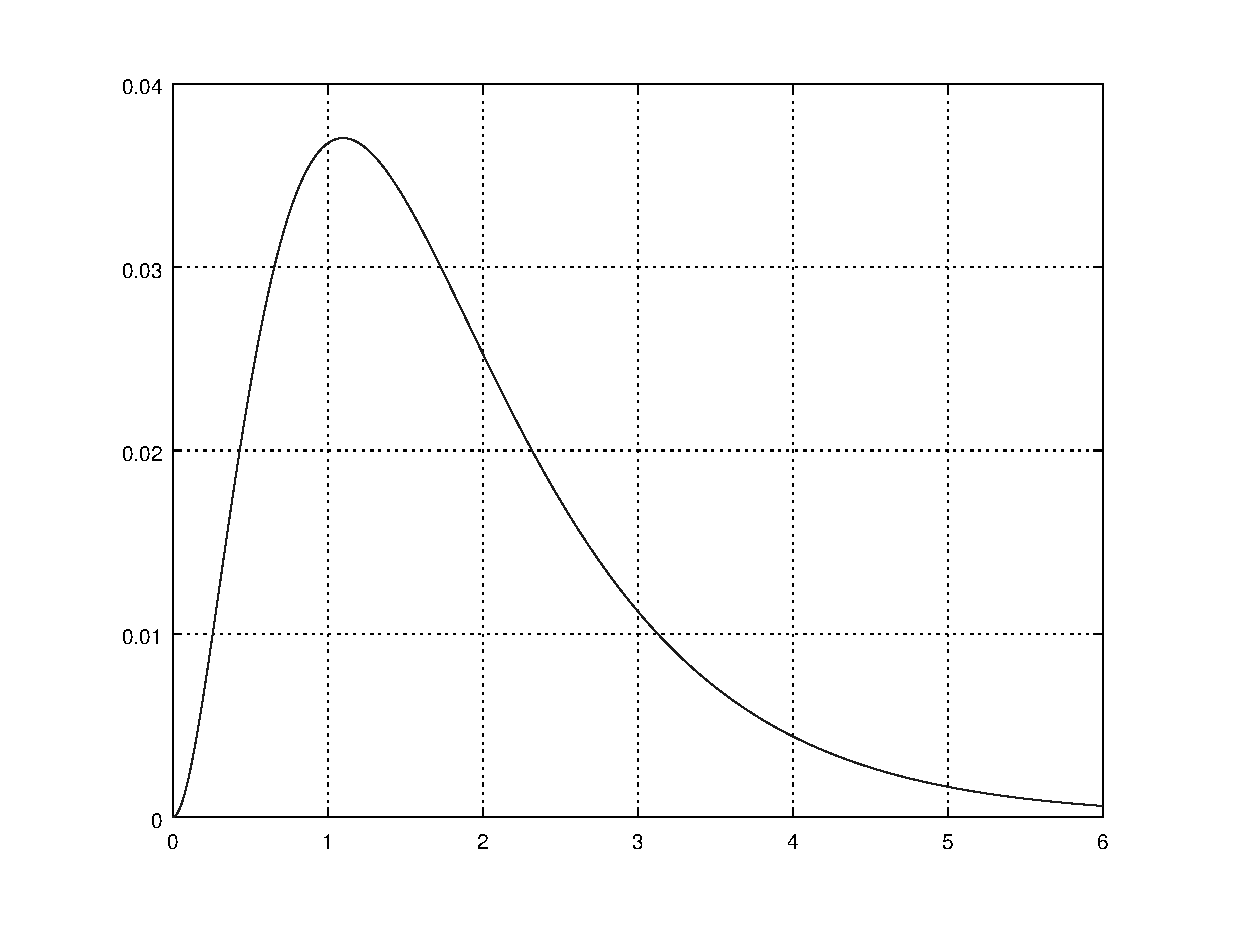
\includegraphics[width=1\linewidth]{./Ejercicio2/resp_impulso}
            \caption{Respuesta obtenida por el equipo}
          \end{center}
        \end{subfigure}%    
        \begin{subfigure}{0.5\textwidth}
          \begin{center}
            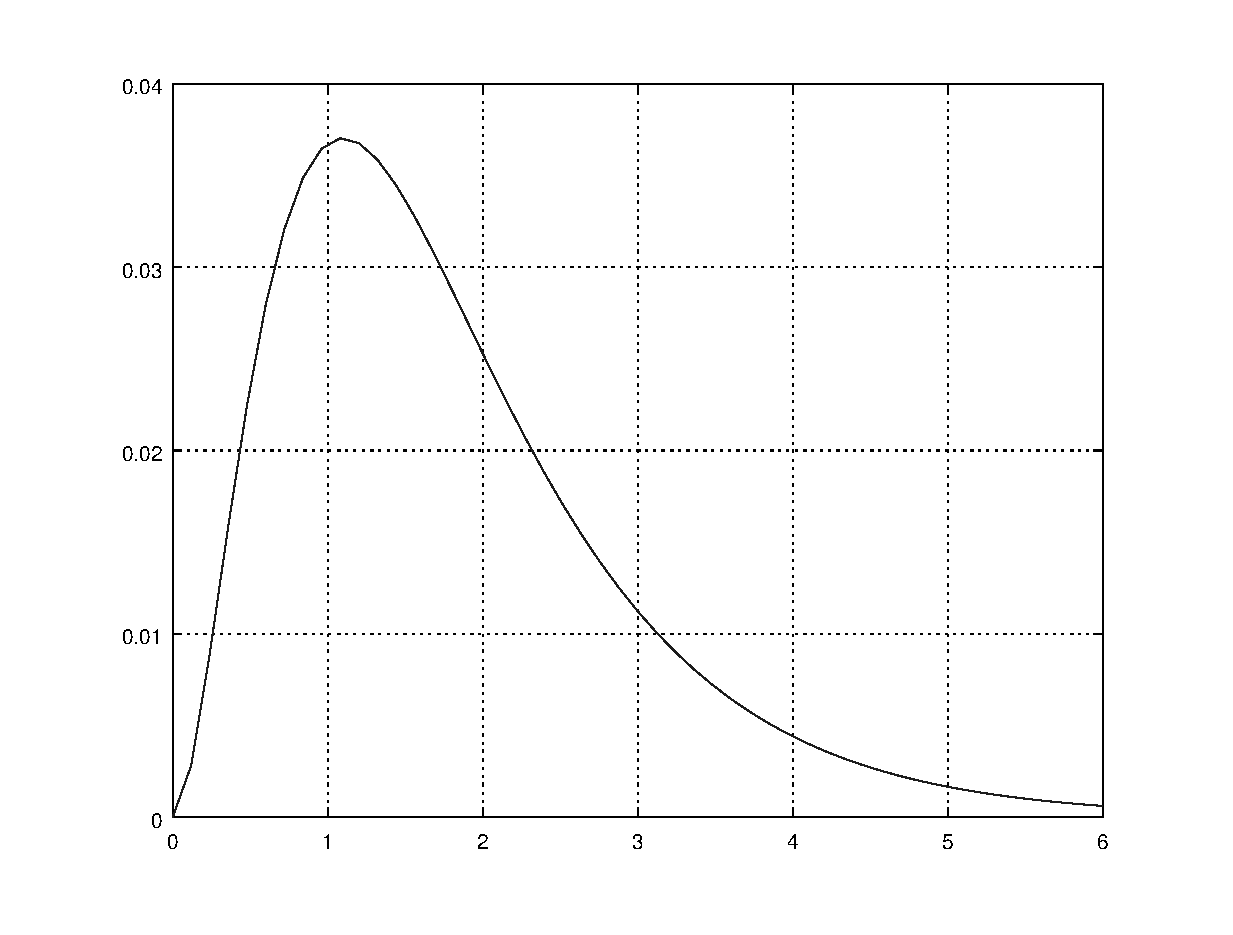
\includegraphics[width=1\linewidth]{./Ejercicio2/resp_impulso_matlab}
            \caption{Respuesta al impulso de Matlab}
          \end{center}
        \end{subfigure}
        \caption{Respuesta al impulso del sistema}
        \label{resp_impulso}
      \end{center}
    \end{figure}
    Código en Matlab \texttt{Figura \ref{resp_impulso}(a)}:
    \lstinputlisting{./Ejercicio2/resp_impulso.m}
    Código en Matlab \texttt{Figura \ref{resp_impulso}(b)}:
    \lstinputlisting{./Ejercicio2/resp_impulso_matlab.m}
    \newpage
  \item[c)] La respuesta al escalón\\
    Suponiendo condiciones iniciales nulas:
    \[ Y\left(s\right) = \frac{\frac{1}{2}}{\left(s^3 + 6s^2 + 11s + 6\right)s} = \frac{A}{s} + \frac{B}{s + 1} + \frac{C}{s + 2} + \frac{D}{s + 3} \]
    \[ A = \frac{1}{12} \quad ; \quad B = -\frac{1}{4} \quad ; \quad C = \frac{1}{4} \quad ; \quad D = -\frac{1}{12} \]
    \[ \mathcal{L}^{-1} \left\{ \frac{\frac{1}{12}}{s} + \frac{-\frac{1}{4}}{s + 1} + \frac{\frac{1}{4}}{s + 2} + \frac{-\frac{1}{12}}{s + 3} \right\} \]
    \[ y\left(t\right) = \left( \frac{1}{12} - \frac{1}{4}e^{-t} + \frac{1}{4}e^{-2t} - \frac{1}{12}e^{-3t} \right) u\left(t\right) \]
    \begin{figure}[H]
      \begin{center}    
        \begin{subfigure}{0.5\textwidth}
          \begin{center}
            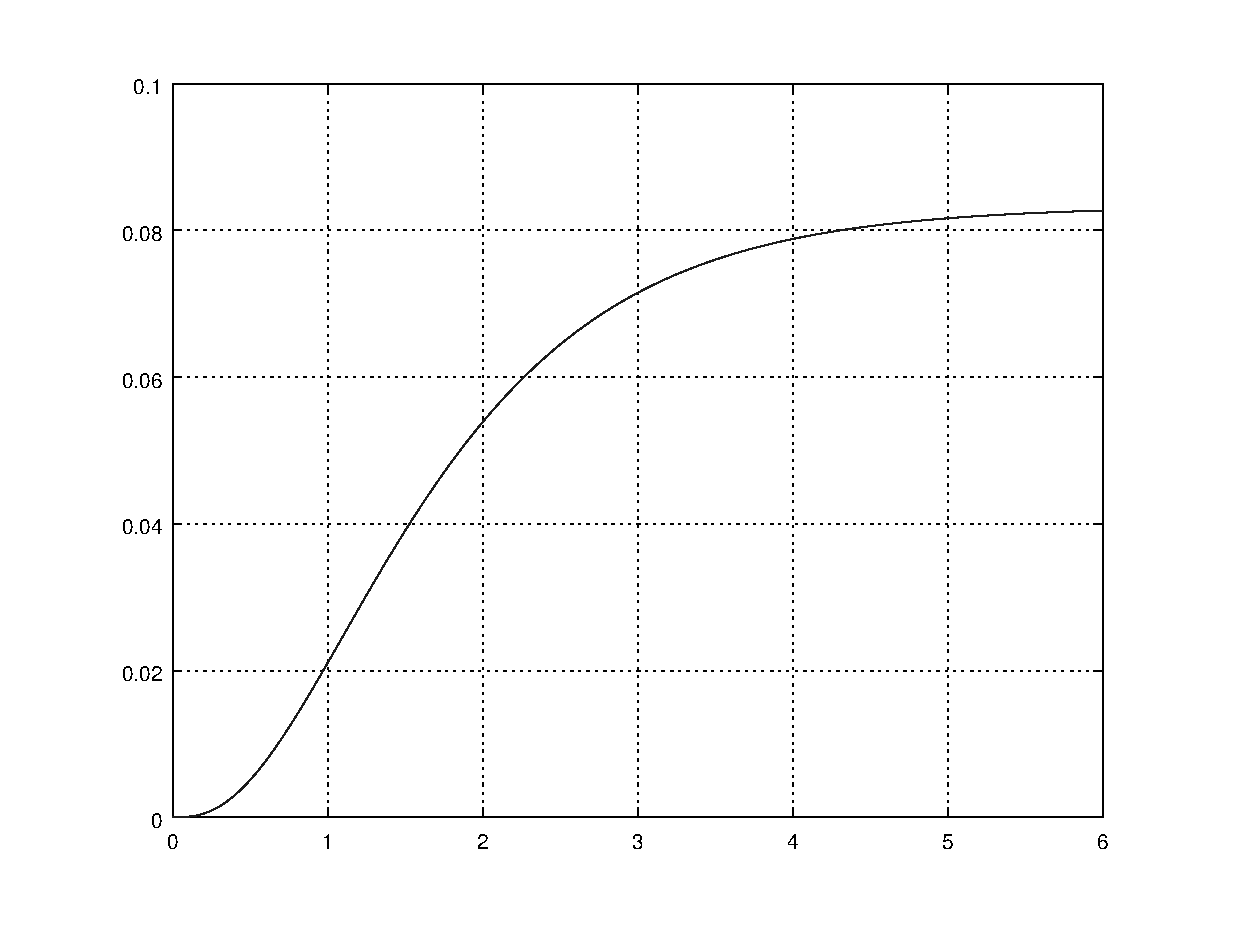
\includegraphics[width=1\linewidth]{./Ejercicio2/resp_escalon}
            \caption{Respuesta al escalón obtenida por el equipo}
          \end{center}
        \end{subfigure}%    
        \begin{subfigure}{0.5\textwidth}
          \begin{center}
            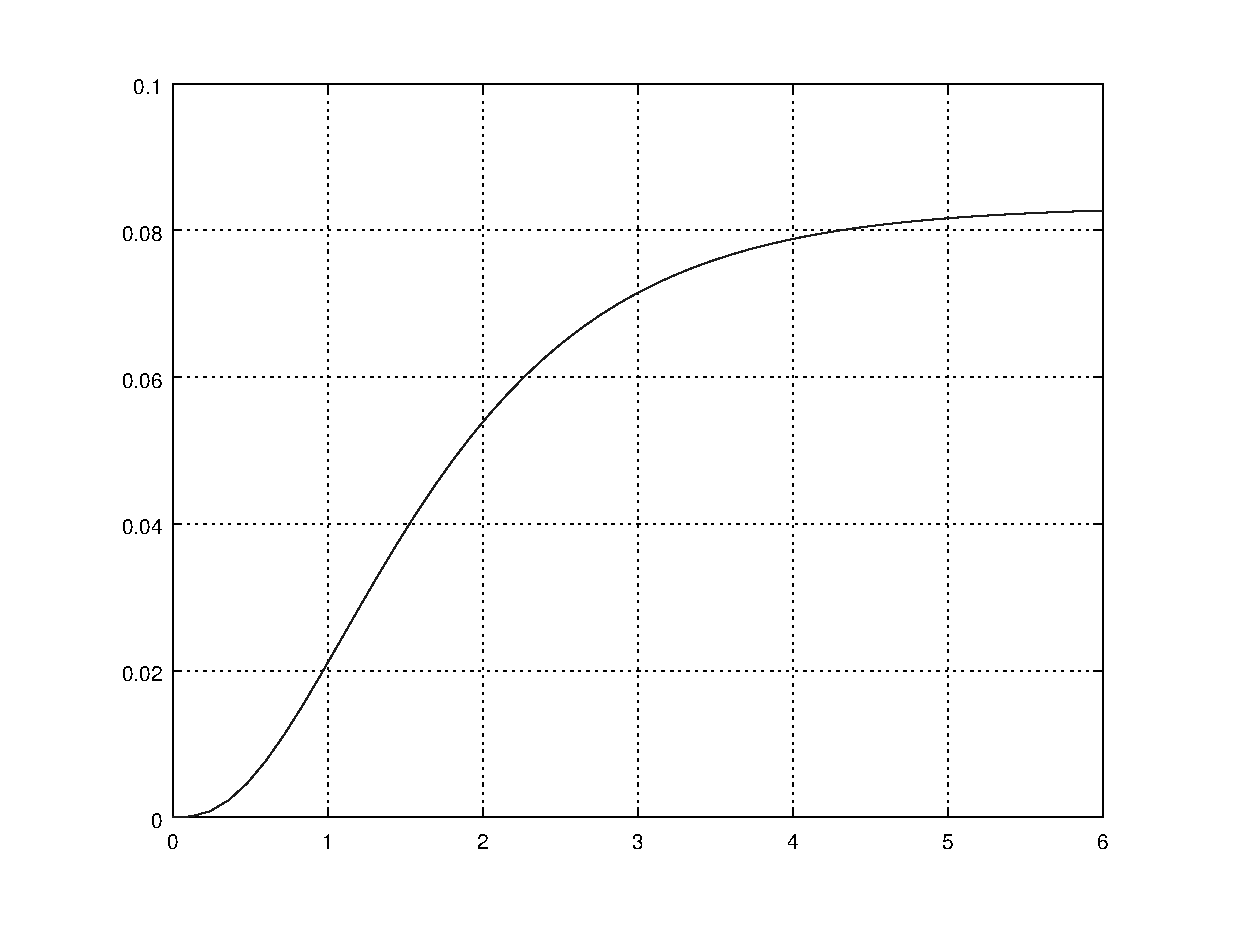
\includegraphics[width=1\linewidth]{./Ejercicio2/resp_escalon_matlab}
            \caption{Respuesta al escalón de Matlab}
          \end{center}
        \end{subfigure}
        \caption{Respuesta al escalón del sistema}
        \label{resp_escalon}
      \end{center}
    \end{figure}
    Código en Matlab \texttt{Figura \ref{resp_escalon}(a)}:
    \lstinputlisting{./Ejercicio2/resp_escalon.m}
    Código en Matlab \texttt{Figura \ref{resp_escalon}(b)}:
    \lstinputlisting{./Ejercicio2/resp_escalon_matlab.m}
  \item[d)] El diagrama de polos y ceros y diga si es estable o no.\\
    Del inciso anterior, suponiendo condiciones iniciales nulas, los polos del sistema están en $-1, -2, -3$ y no tiene ceros, dado que todas sus raíces están en el semiplano izquierdo, el sistema es estable.
    \begin{figure}[H]
      \begin{center}
        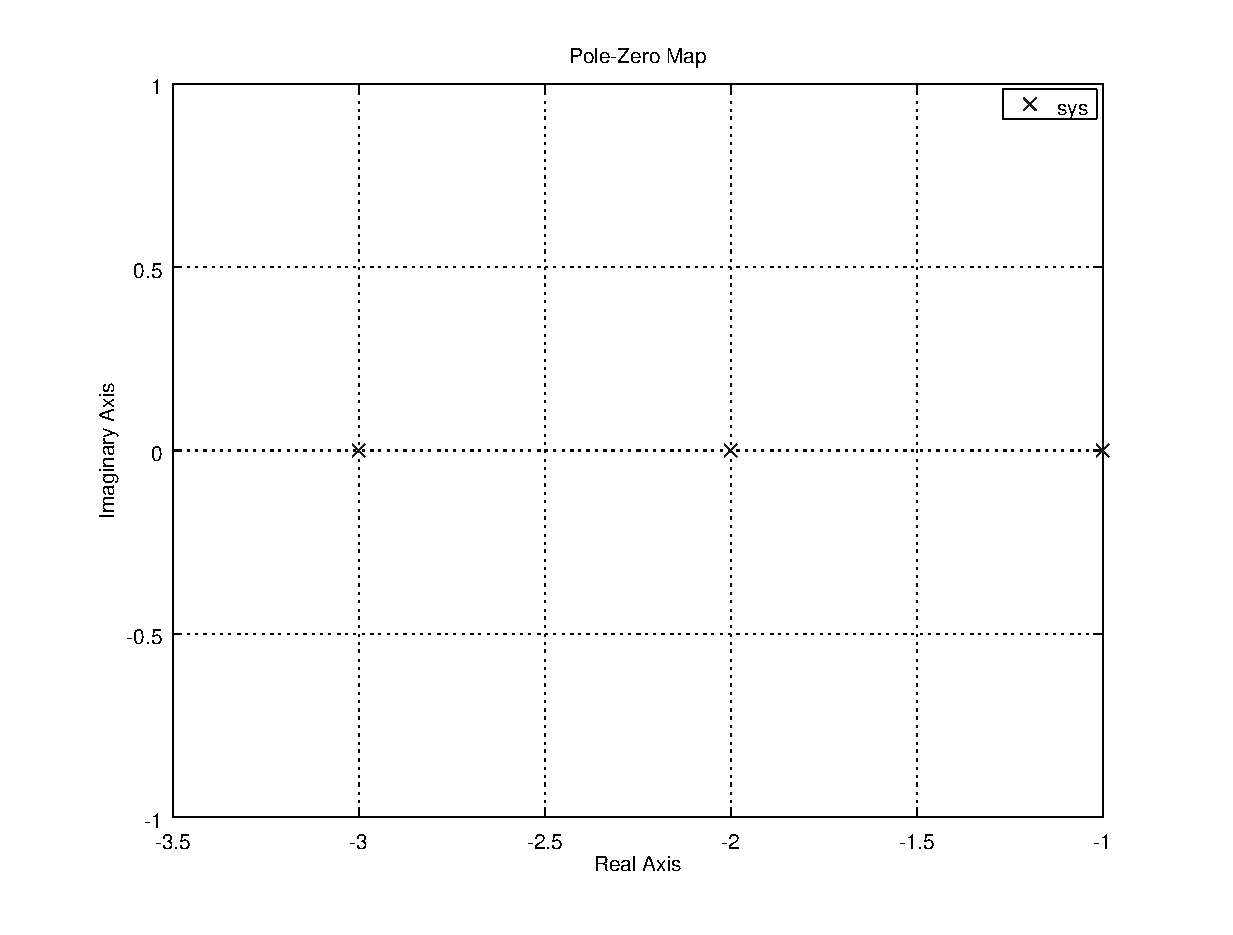
\includegraphics[width=0.6\textwidth]{./Ejercicio2/polos_zeros}
        \caption{Diagrama de polos y ceros}
      \end{center}
    \end{figure}
    Código en Matlab:
    \lstinputlisting{./Ejercicio2/polos_zeros.m}
\end{enumerate}

\section{Ejercicio 3}
Considerando el ejercicio práctico realizado en el laboratorio:
\begin{enumerate}
  \item[a)] Determine la respuesta al impulso y la respuesta al escalón con tres valores del factor de amortiguamiento $\zeta$ y grafique las respuestas.
    \begin{figure}[H]
      \begin{center}
        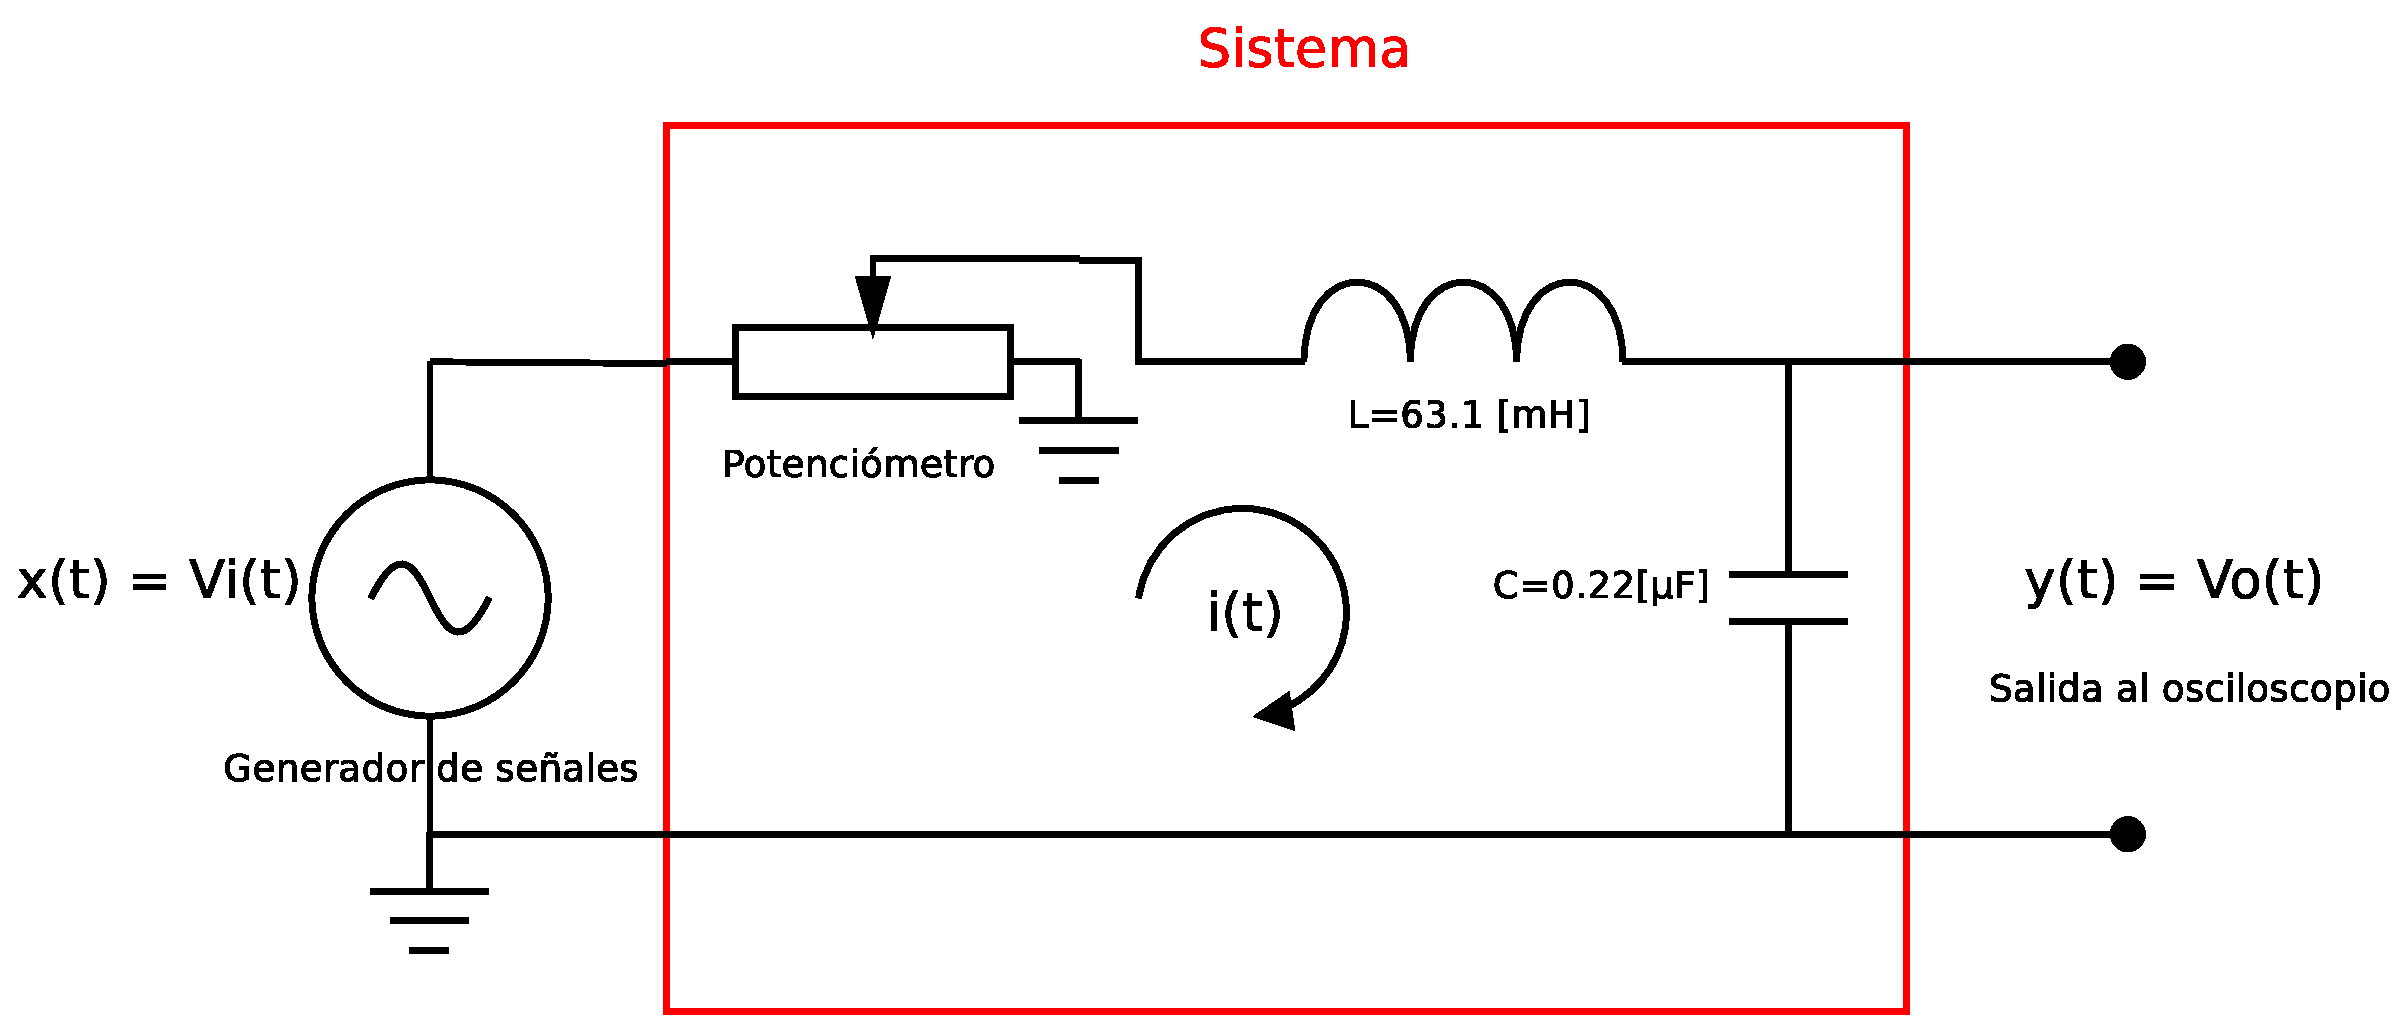
\includegraphics[width=0.6\textwidth]{./Ejercicio3/Diagrama1}
        \caption{Modelo del sistema}
      \end{center}
    \end{figure}
\end{enumerate}
    Conocemos la expresión matemática del modelo del sistema:
    \[ V_o\left(t\right)= L\frac{di\left(t\right)}{dt} + R_{eq}i\left(t\right) + \frac{1}{C}\int i\left(t\right)dt \]
    donde:
    \[ i(t) = C\frac{dV_i\left(t\right)}{dt} \]
    Transformando tenemos
    \[ \mathcal{L} \left\{ V_o\left(t\right)= L\frac{di\left(t\right)}{dt} + R_{eq}i\left(t\right) + \frac{1}{C}\int i\left(t\right)dt \right\} \quad ; \quad \mathcal{L} \left\{ i\left(t\right) = C\frac{dV_i\left(t\right)}{dt} \right\} \]
    \[ V_o\left(s\right)= LsI\left(s\right) + R_{eq}I\left(s\right) + \frac{1}{sC}I\left(s\right) \quad ; \quad I\left(s\right) = CsV_i\left(t\right) \]
    Sustituyendo $I\left(s\right)$ tenemos:
    \[ V_o\left(s\right)= LCs^2V_i\left(t\right) + R_{eq}CsV_i\left(t\right) + V_i\left(t\right) \]
    La función de transferencia es entonces:
    \[ H\left(s\right) = \frac{V_o\left(s\right)}{V_i\left(s\right)} = \frac{1}{LCs^2 + R_{eq}Cs + 1} = \frac{\frac{1}{LC}}{s^2 + \frac{R_{eq}}{L}s + \frac{1}{LC}} \]
    Comparándola con la expresión general de la función de transferencia para modelos de segundo orden, llegamos a algunas conclusiones:
    \[\begin{split}
      H\left(s\right) &= \frac{k}{s^2 + 2\zeta \omega_ns + \omega_n^2}\\
      k &= \frac{1}{LC}\\
      \omega_n^2 &= \frac{1}{LC} \quad ; \quad \omega_n = \frac{1}{\sqrt{LC}}\\
      2 \zeta \omega_n &= 2\zeta\frac{1}{\sqrt{LC}} = \frac{R_{eq}}{2L} \quad ; \quad \zeta = \frac{R_{eq}}{2}\sqrt{\frac{C}{L}}
    \end{split}\]
    Si sabemos que $L = 0.0631 \left[H\right]$, $C=2.2x10^{-7}\left[F\right]$, y que debido a las resistencias aportadas por el osciloscopio y la bobina, nunca se alcanzará un valor de $0\left[\Omega\right]$ para la $R_{eq}$, tenemos sólo distintas 3 respuestas de acuerdo al valor de la resistencia equivalente:
    \[\begin{split}
      &\text{Caso 1} \qquad \zeta = 1 \quad ; \quad R_{eq} = 2\sqrt{\frac{L}{C}} \quad ; \quad R_{eq} = 1071.1\left[\Omega\right]\\
      &\text{Caso 2} \qquad 0 < \zeta < 1 \quad ; \quad 0\left[\Omega\right]  < R_{eq} < 1071.1\left[\Omega\right] \quad\\
      &\text{Caso 3} \qquad \zeta > 1 \quad ; \quad R_{eq} > 1071.1\left[\Omega\right] \quad
    \end{split}\]
    Respuestas al impulso:
    \begin{itemize}
      \item Caso 1:\\
      Suponiendo $\zeta = 1$
      \[ H\left(s\right) = \frac{72035730}{s^2 + 16975s + 72035730} \]
      Antitransformando:
      \[ h\left(t\right) = \left( 820660e^{-8443.6t} -820660e^{-8531.4t} \right) u\left(t\right) \]
      Código en Matlab:
      \lstinputlisting{./Ejercicio3/resp_impulso_1.m}
      \begin{figure}[H]
        \begin{center}
          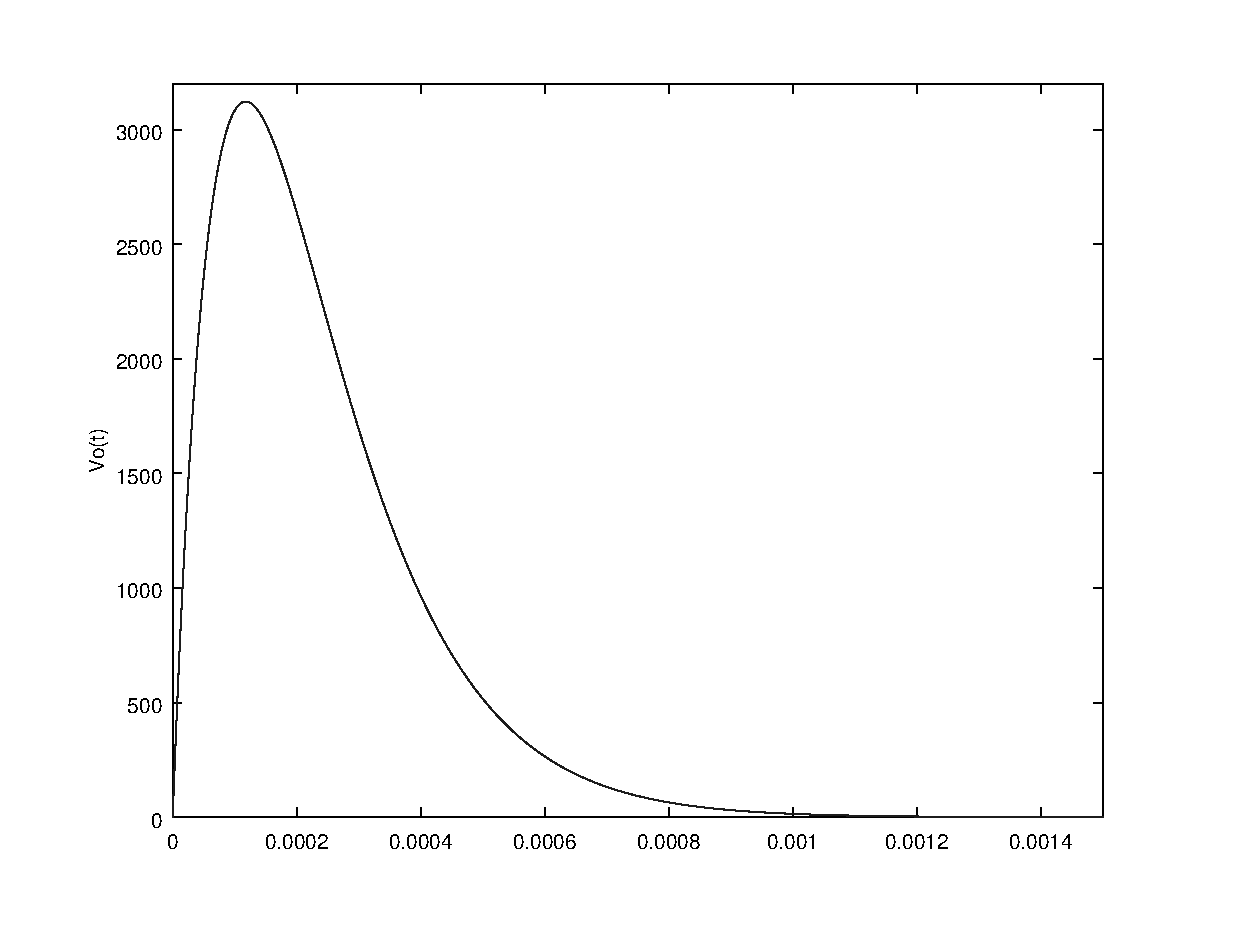
\includegraphics[width=0.6\textwidth]{./Ejercicio3/resp_impulso_1}
          \caption{Respuesta al impuso para $\zeta = 1$}
        \end{center}
      \end{figure}
    
      \item Caso 2:\\
        Suponiendo $\zeta = 0.5$
        \[ H\left(s\right) = \frac{72035730}{s^2 + 8487s + 72035730} \]
        Antitransformando:
        \[ h\left(t\right) = \left(4900.1ie^{\left(-4243.5 - 7350.4i\right)t} - 4900.1ie^{\left(-4243.5 + 7350.4i\right)t} \right) u\left(t\right) \]
        Código en Matlab:
        \lstinputlisting{./Ejercicio3/resp_impulso_2.m}
        \begin{figure}[H]
          \begin{center}
            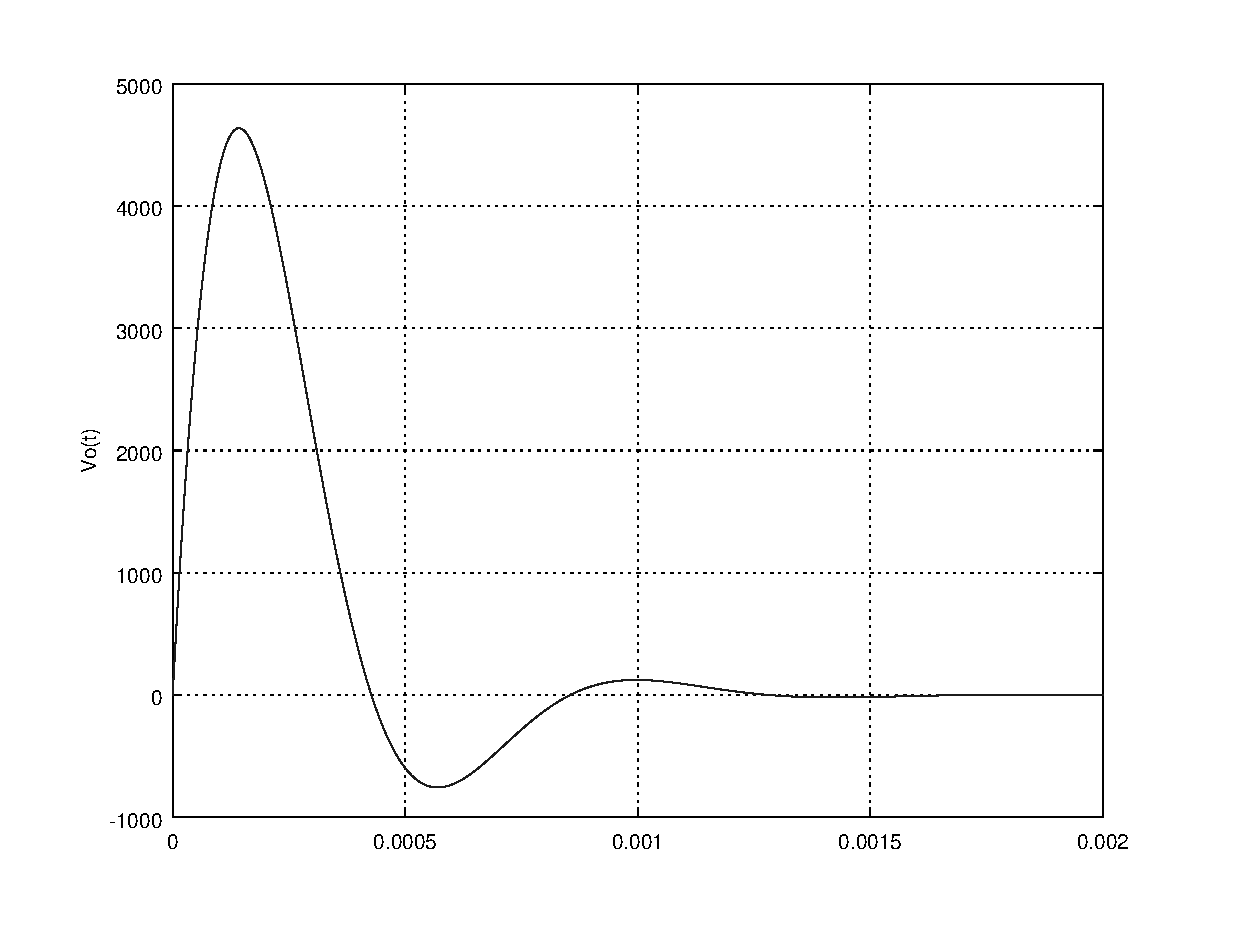
\includegraphics[width=0.6\textwidth]{./Ejercicio3/resp_impulso_2}
            \caption{Respuesta al impuso para $\zeta = 0.5$}
          \end{center}
        \end{figure}
      \item Caso 3:
        Suponiendo $\zeta = 1.5$
        \[ H\left(s\right) = \frac{72035730}{s^2 + 25462s + 72035730} \]
        Antitransformando:
        \[ h\left(t\right) = \left(3795.7e^{\left(-3241.9\right)t} - 3795.7e^{\left(-22220\right)t} \right) u\left(t\right) \]
        Código en Matlab:
        \lstinputlisting{./Ejercicio3/resp_impulso_3.m}
        \begin{figure}[H]
          \begin{center}
            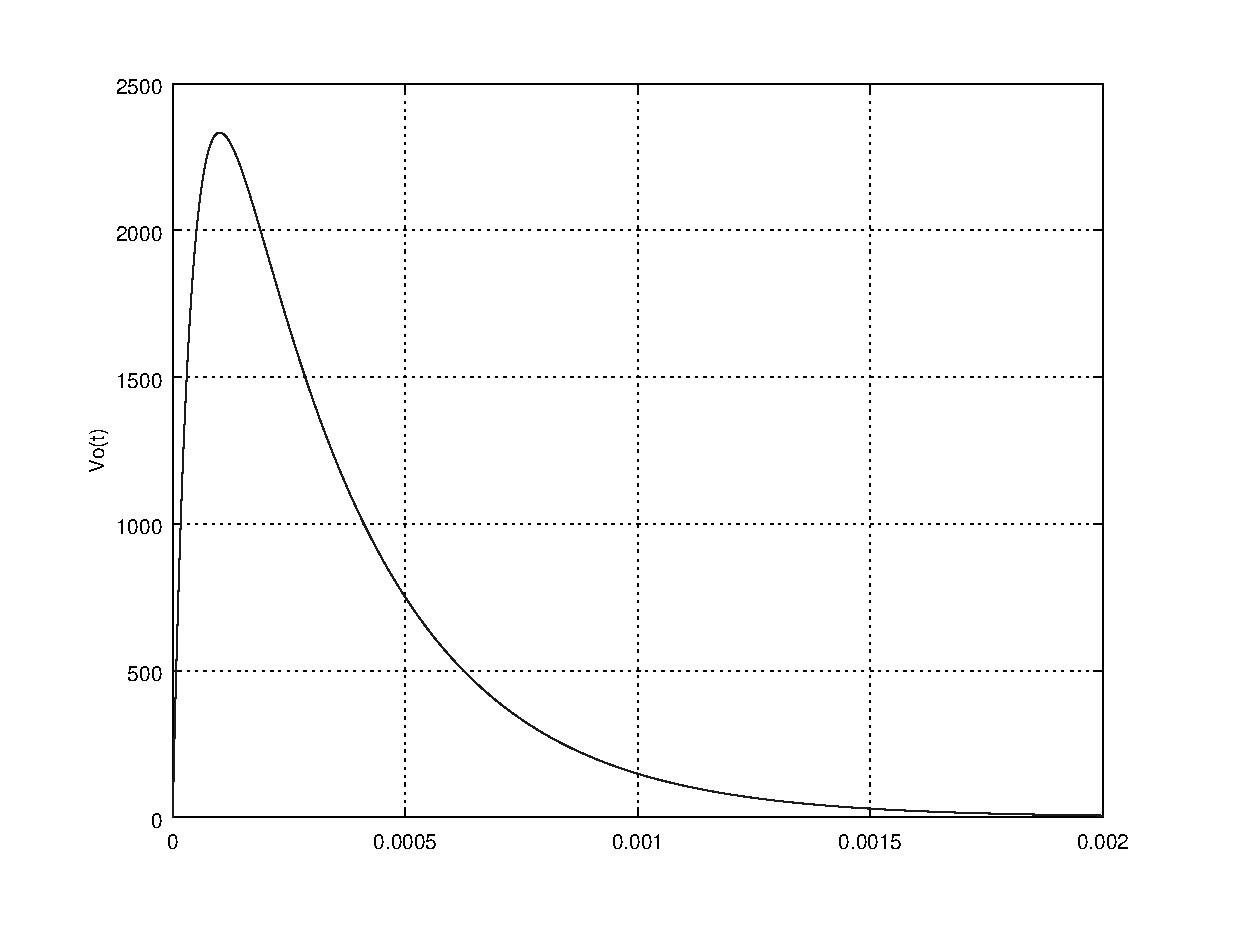
\includegraphics[width=0.6\textwidth]{./Ejercicio3/resp_impulso_3}
            \caption{Respuesta al impuso para $\zeta = 1.5$}
          \end{center}
        \end{figure}
    \end{itemize}
    Respuestas al escalon:
    \begin{itemize}
      \item Caso 1:\\
      Suponiendo $\zeta = 1$
      \[ Y\left(s\right) = \frac{72035730}{s\left(s^2 + 16975s + 72035730\right)} \]
      Antitransformando:
      \[ y\left(t\right) = \left( 1 - 97.1927e^{-8443.6t} + 96.1927e^{-8531.4t} \right) u\left(t\right) \]
      Código en Matlab:
      \lstinputlisting{./Ejercicio3/resp_impulso_1.m}
      \begin{figure}[H]
        \begin{center}
          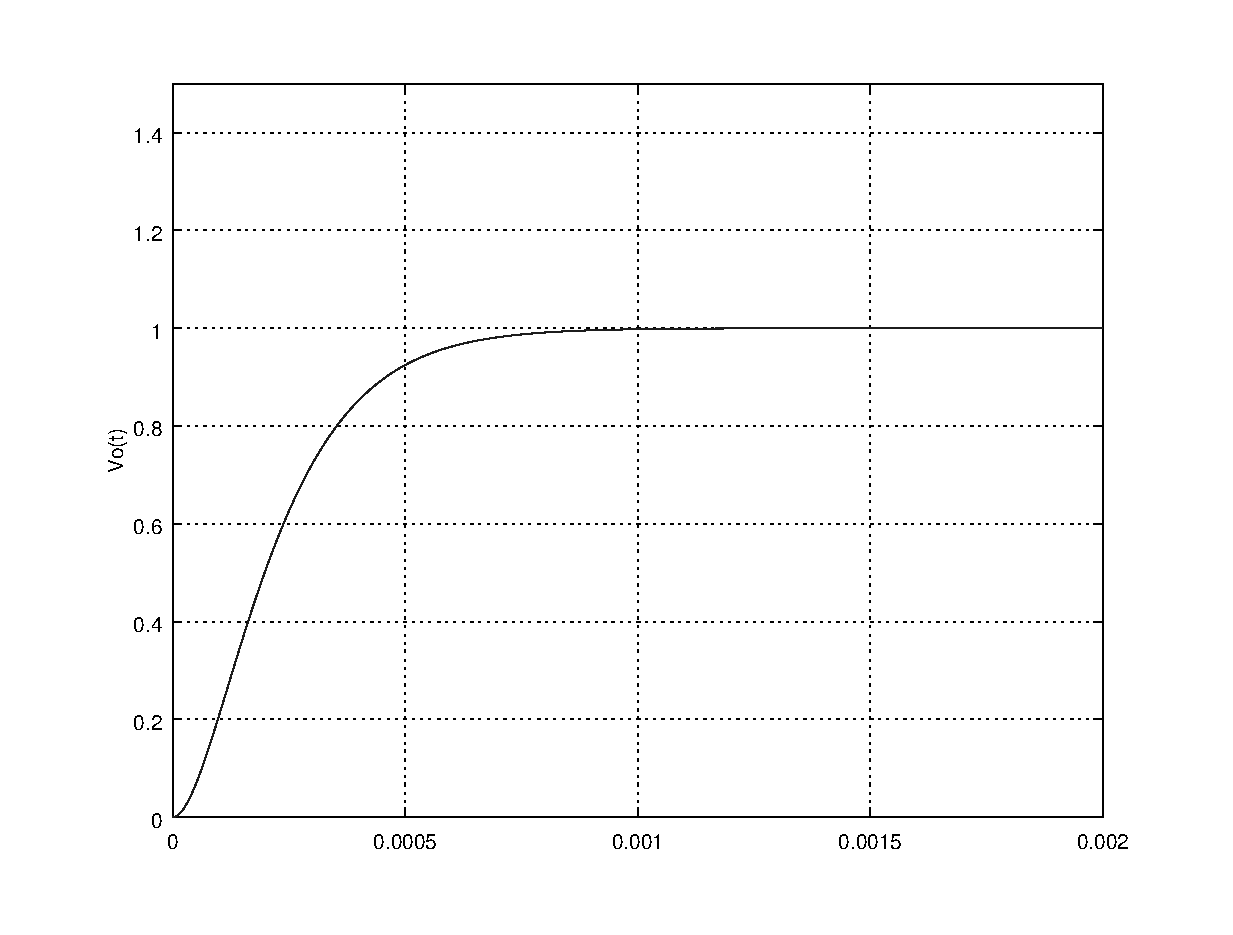
\includegraphics[width=0.6\textwidth]{./Ejercicio3/resp_escalon_1}
          \caption{Respuesta al escalón para $\zeta = 1$}
        \end{center}
      \end{figure}
    
      \item Caso 2:\\
        Suponiendo $\zeta = 0.5$
        \[ Y\left(s\right) = \frac{72035730}{s\left(s^2 + 8487s + 72035730\right)} \]
        Antitransformando:
        \[ y\left(t\right) = \left( 1 + \left(-0.50000 + 0.28866i\right)e^{\left(-4243.5 - 7350.4i\right)t} + \left(-0.50000 - 0.28866i\right)e^{\left(-4243.5 + 7350.4i\right)t} \right) u\left(t\right) \]
        Código en Matlab:
        \lstinputlisting{./Ejercicio3/resp_impulso_2.m}
        \begin{figure}[H]
          \begin{center}
            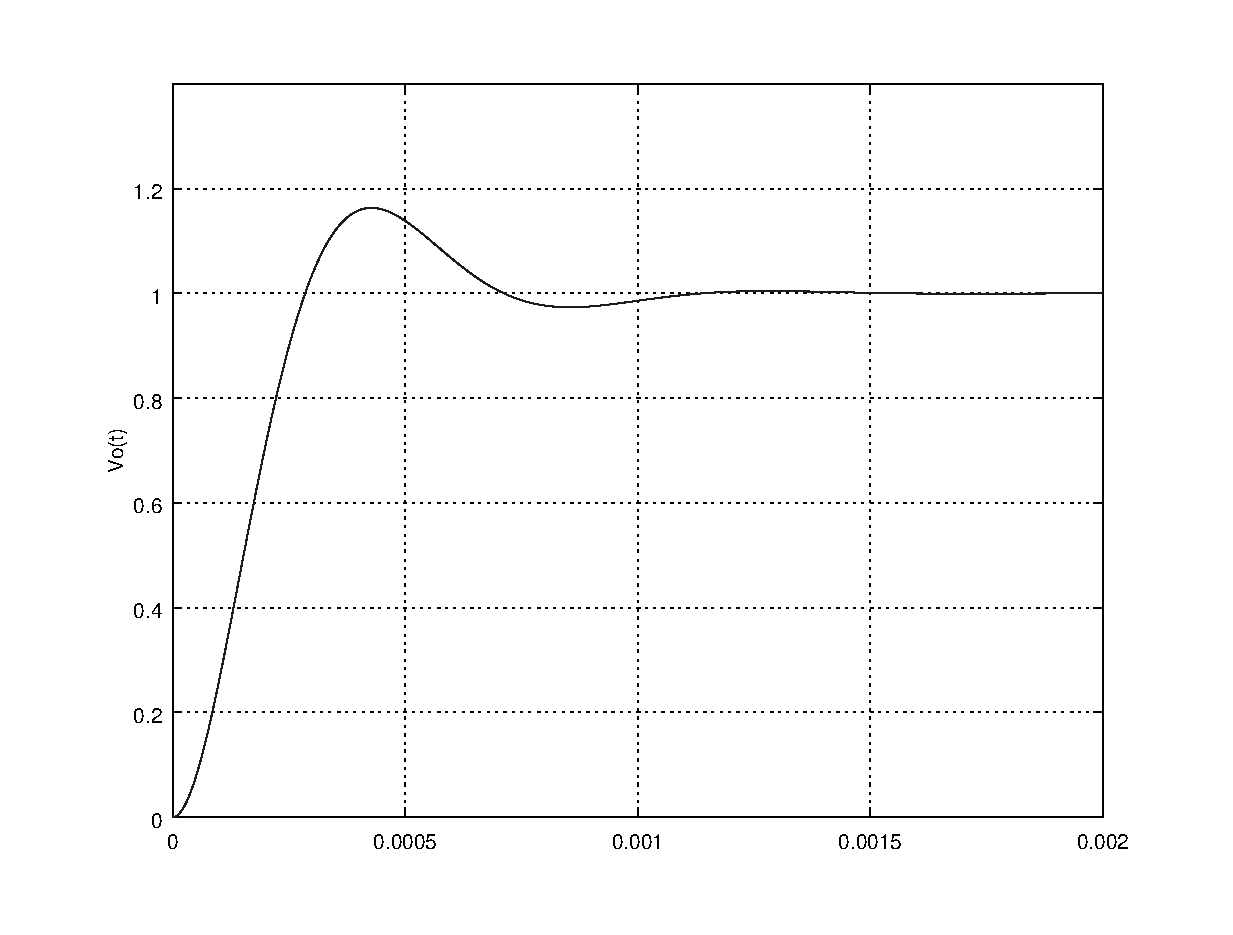
\includegraphics[width=0.6\textwidth]{./Ejercicio3/resp_escalon_2}
            \caption{Respuesta al escalón para $\zeta = 0.5$}
          \end{center}
        \end{figure}
      \item Caso 3:
        Suponiendo $\zeta = 1.5$
        \[ Y\left(s\right) = \frac{72035730}{s\left(s^2 + 25462s + 72035730\right)} \]
        Antitransformando:
        \[ y\left(t\right) = \left( 1 - 1.17082e^{\left(-3241.9\right)t} + 0.17082e^{\left(-22220\right)t} \right) u\left(t\right) \]
        Código en Matlab:
        \lstinputlisting{./Ejercicio3/resp_impulso_3.m}
        \begin{figure}[H]
          \begin{center}
            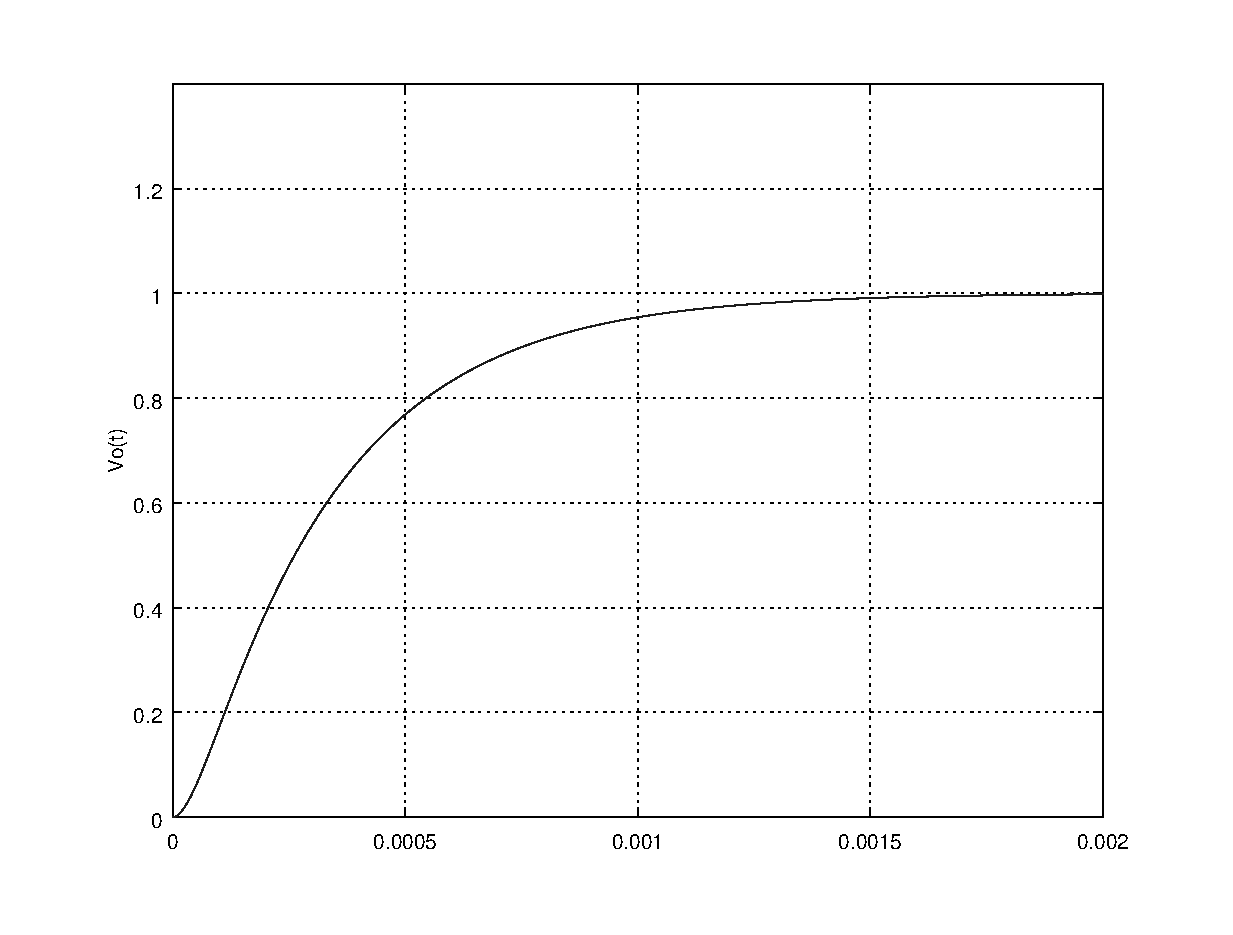
\includegraphics[width=0.6\textwidth]{./Ejercicio3/resp_escalon_3}
            \caption{Respuesta al escalón para $\zeta = 1.5$}
          \end{center}
        \end{figure}
    \end{itemize}
    
    
\section{Ejercicio 4}

\section{Ejercicio 5}
Considere el siguiente sistema:
\[ \frac{{d^2}y}{dt^2} + 4y\left(t\right) = x\left(t\right) \]
Determine la respuesta al escalón mediante la convolución.\\
Para determinar la respuesta al escalón requerimos primero conocer la respuesta al impulso $h\left(t\right)$, para ello utilizaremos la transformada de Laplace.
%\[ \mathcal{L} \left\{ \frac{{d^2}y}{dt^2} + 4y\left(t\right) = x\left(t\right) \right\} = s^2Y\left(s\right) + 4Y\left(s\right) = 1 \]
\[ H\left(s\right) = \frac{Y\left(s\right)}{X\left(s\right)} = \frac{1}{s^2 + 4} = \frac{2}{s^2 +4}\left(\frac{1}{2}\right) \]
\[ h\left(t\right) = \mathcal{L}^{-1} \left\{ \frac{2}{s^2 +4}\left(\frac{1}{2}\right) \right\} = \left(\frac{1}{2}\right) sen\left(2t\right) u\left(t\right) \]
Una vez obtenemos $h\left(t\right)$ procedemos a convolucionar.
\[
  \begin{split}
    h\left(t\right) \ast u\left(t\right) & =  \frac{1}{2} \int_{0}^{t} sen\left(2\tau\right) u\left(\tau\right) u\left(t - \tau\right) d\tau\\
    u\left(t\right) = \;\left\{\begin{array}{lc}
                        1 & t\geq0 \\
                        0 & t < 0 \\ 
                      \end{array}\right.
    &\quad ; \quad u\left(t -\tau\right) = \;\left\{\begin{array}{lc}
                        1 & \tau \leq t\\
                        0 & \tau > t \\ 
                      \end{array}\right.\\
    & = \frac{1}{2} \int_{0}^{t} sen\left(2\tau\right)  d\tau = -\frac{1}{4}cos\left(2\tau\right)\left|\begin{array}{l}^{\tau = t}\\_{\tau = 0}\end{array}\right.\\
    & =  \left( \frac{1}{4} - \frac{1}{4}cos\left(2t\right) \right)u\left(t\right)
  \end{split}
\]

\section{Ejercicio 6}
A partir del diagrama de bloques mostrado, obtenga el modelo del sistema en el dominio del tiempo.
\begin{figure}[H]
  \begin{center}
  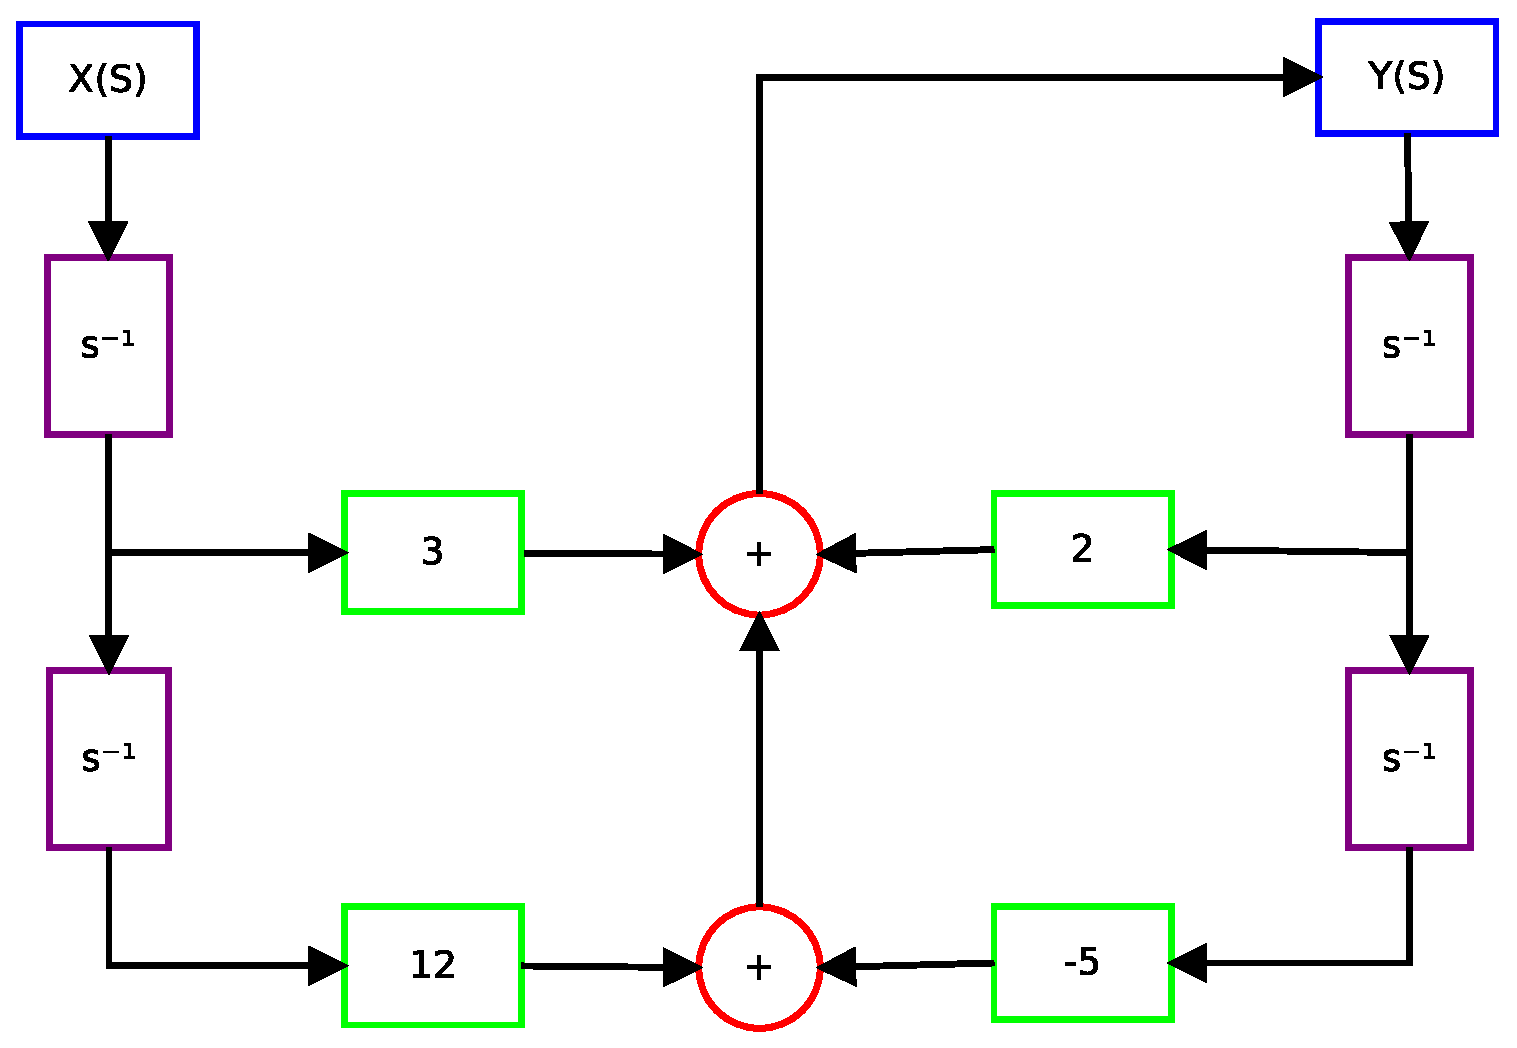
\includegraphics[width=0.4\textwidth]{./Ejercicio6/Diagrama1}
  \caption{Diagrama de bloques del sistema}
  \end{center}
\end{figure}
Analizando el diagrama de bloques
\begin{figure}[H]
      \begin{center}    
        \begin{subfigure}{0.4\textwidth}
          \begin{center}
            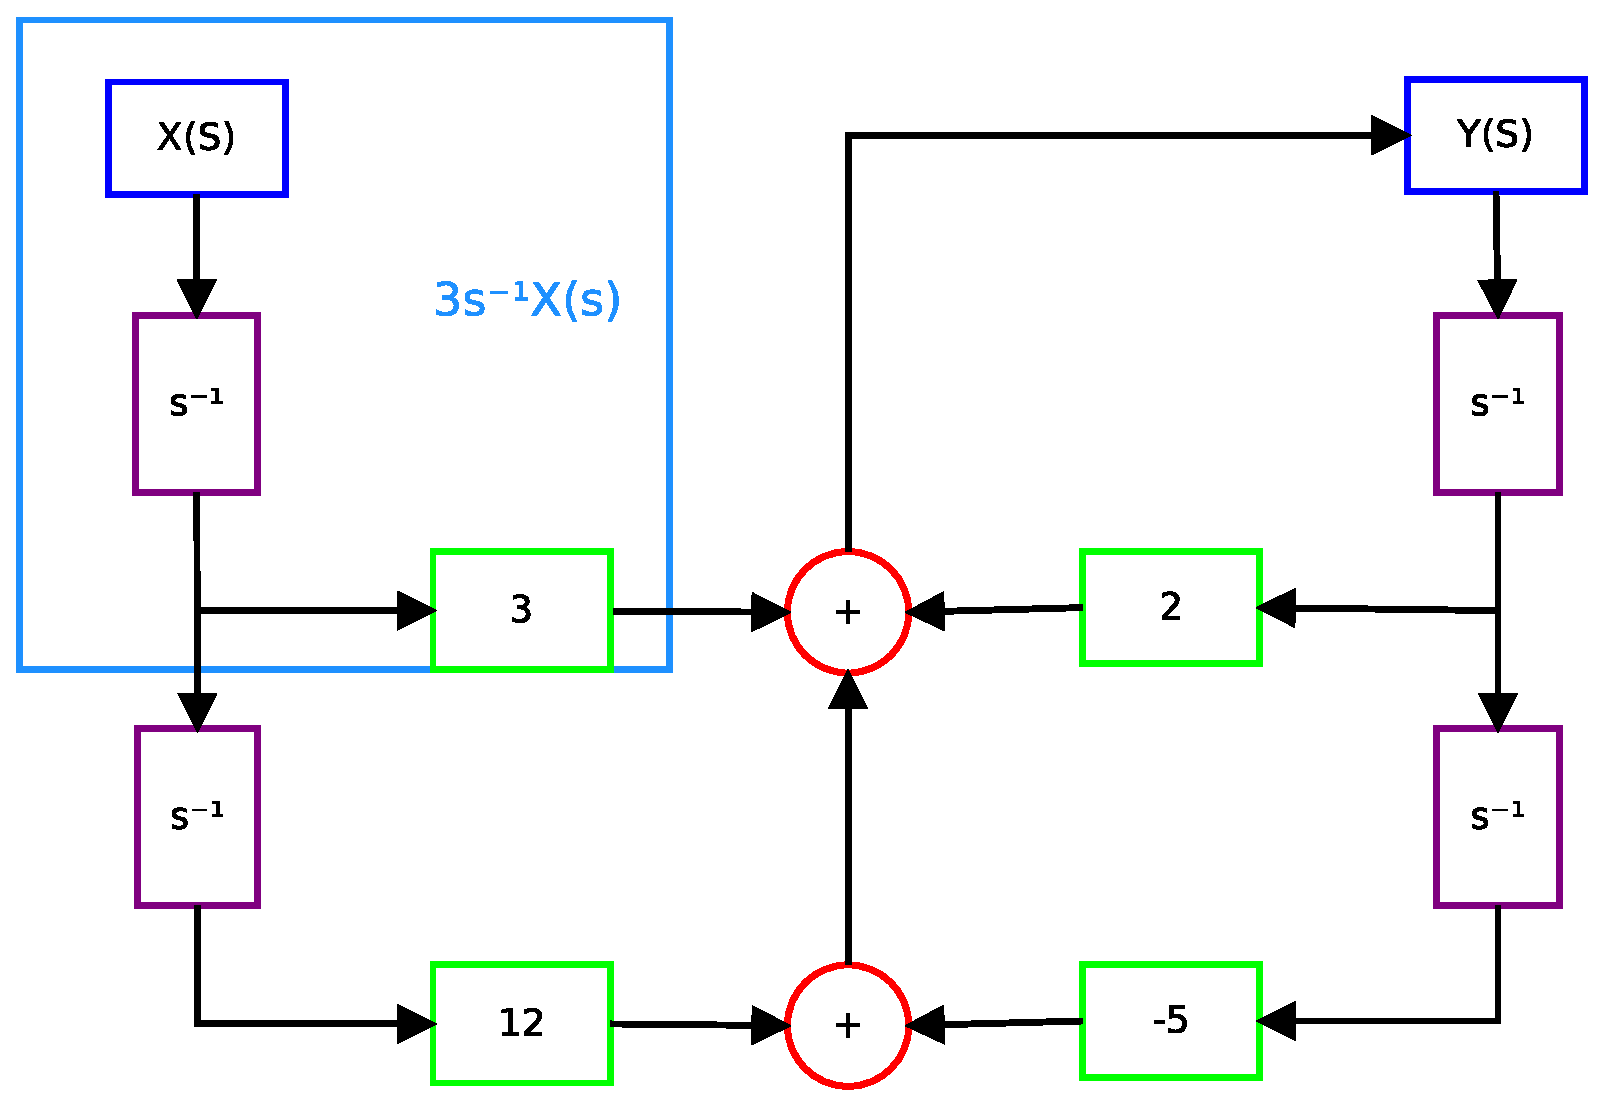
\includegraphics[width=1\linewidth]{./Ejercicio6/Diagrama1_parte1}
          \end{center}
        \end{subfigure}%    
        \begin{subfigure}{0.4\textwidth}
          \begin{center}
            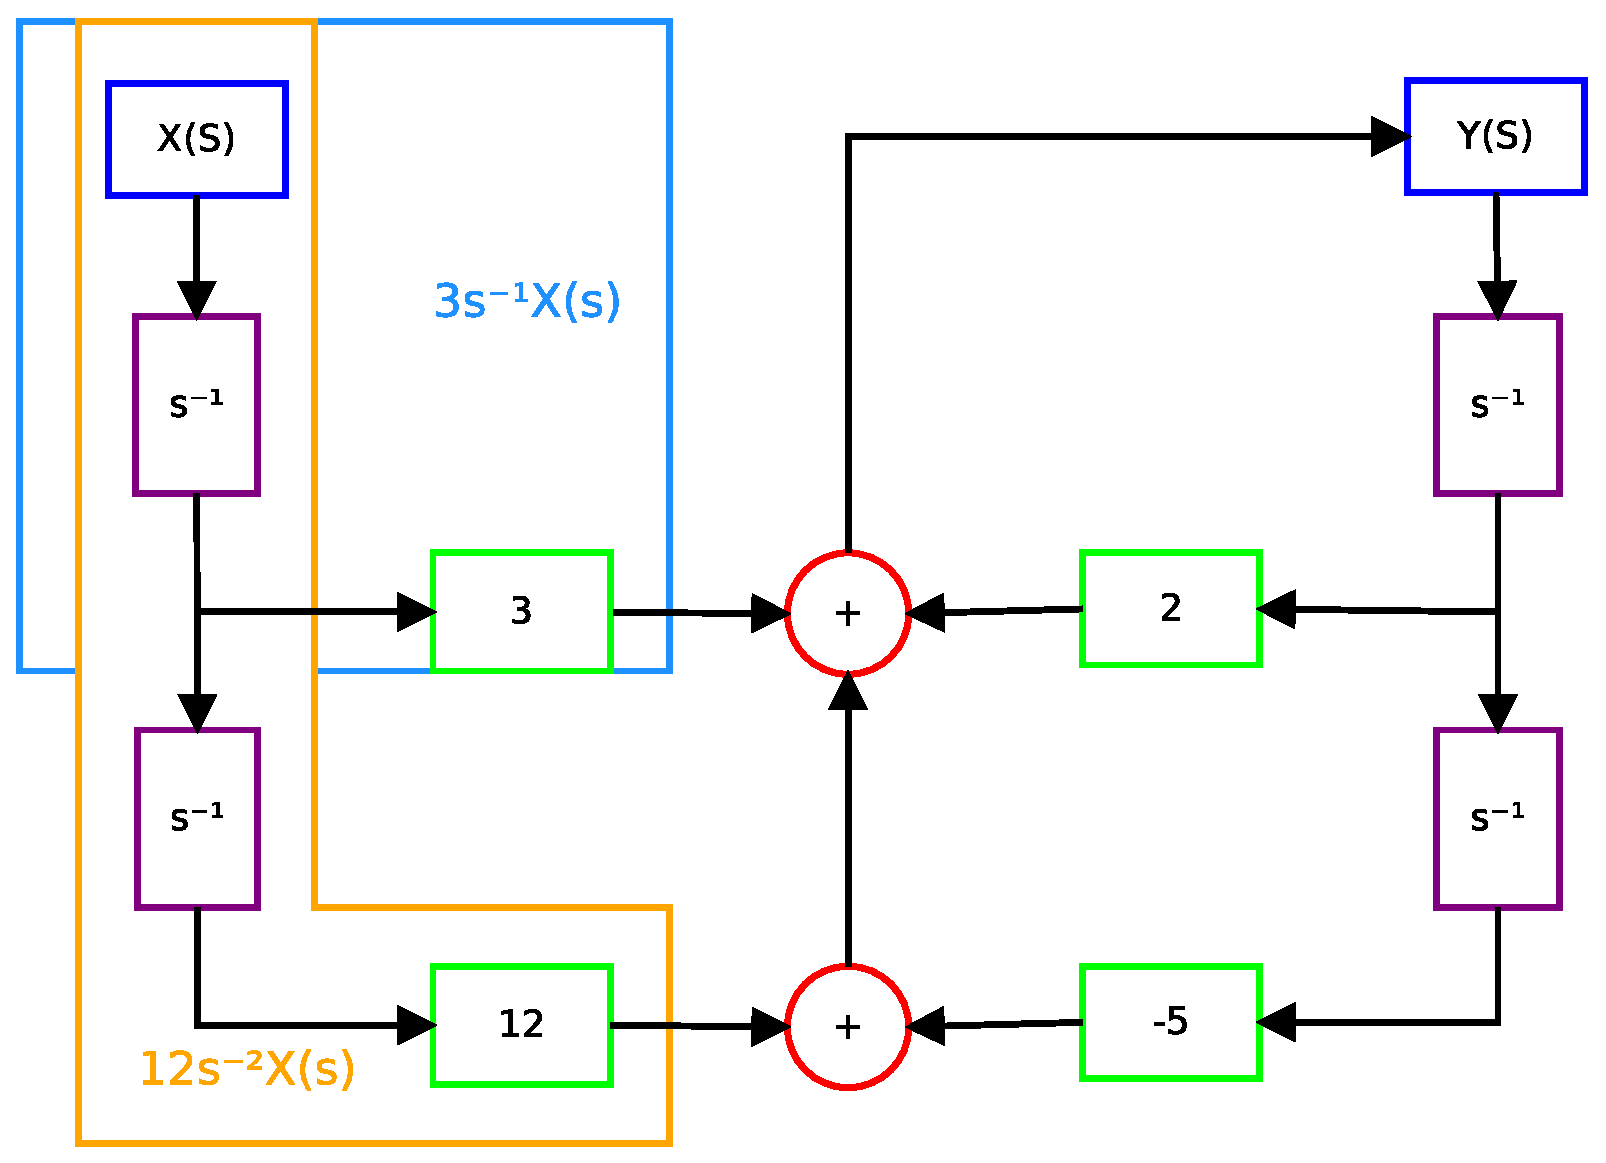
\includegraphics[width=1\linewidth]{./Ejercicio6/Diagrama1_parte2}
          \end{center}
        \end{subfigure}
        \begin{subfigure}{0.4\textwidth}
          \begin{center}
            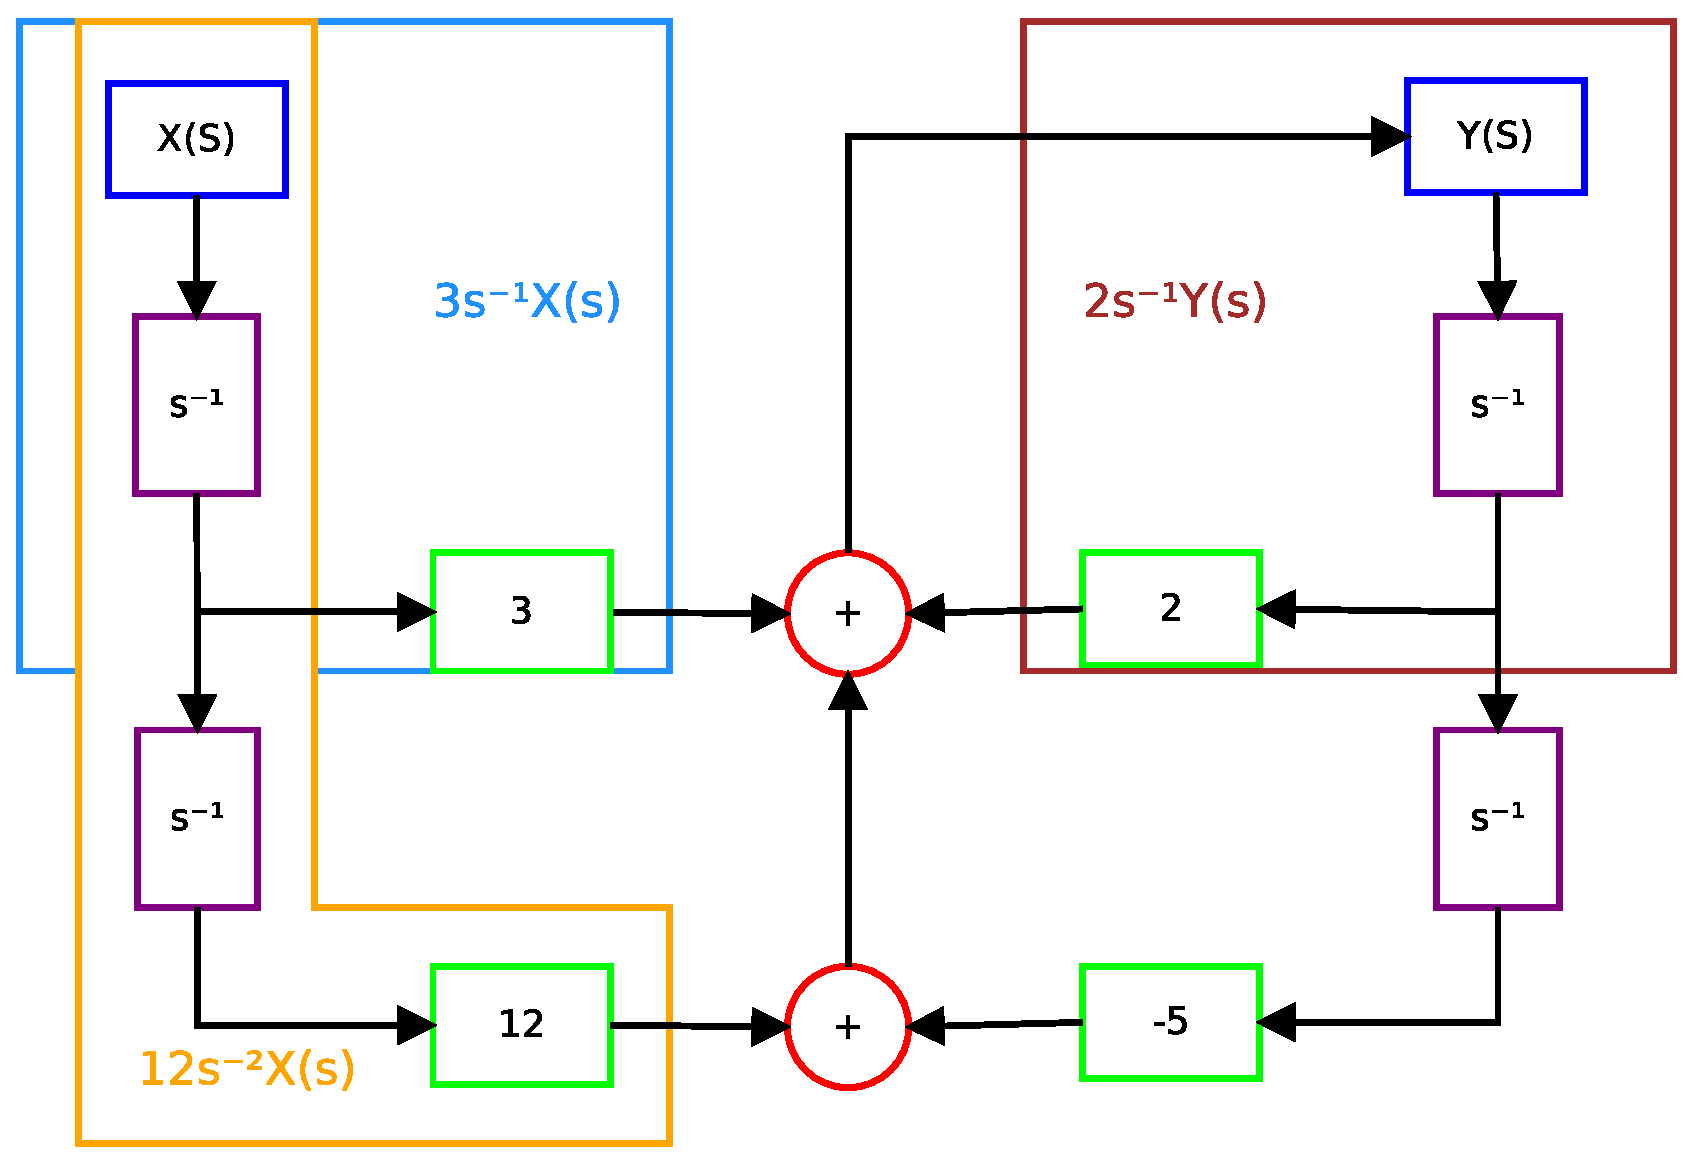
\includegraphics[width=1\linewidth]{./Ejercicio6/Diagrama1_parte3}
          \end{center}
        \end{subfigure}
        \begin{subfigure}{0.4\textwidth}
          \begin{center}
            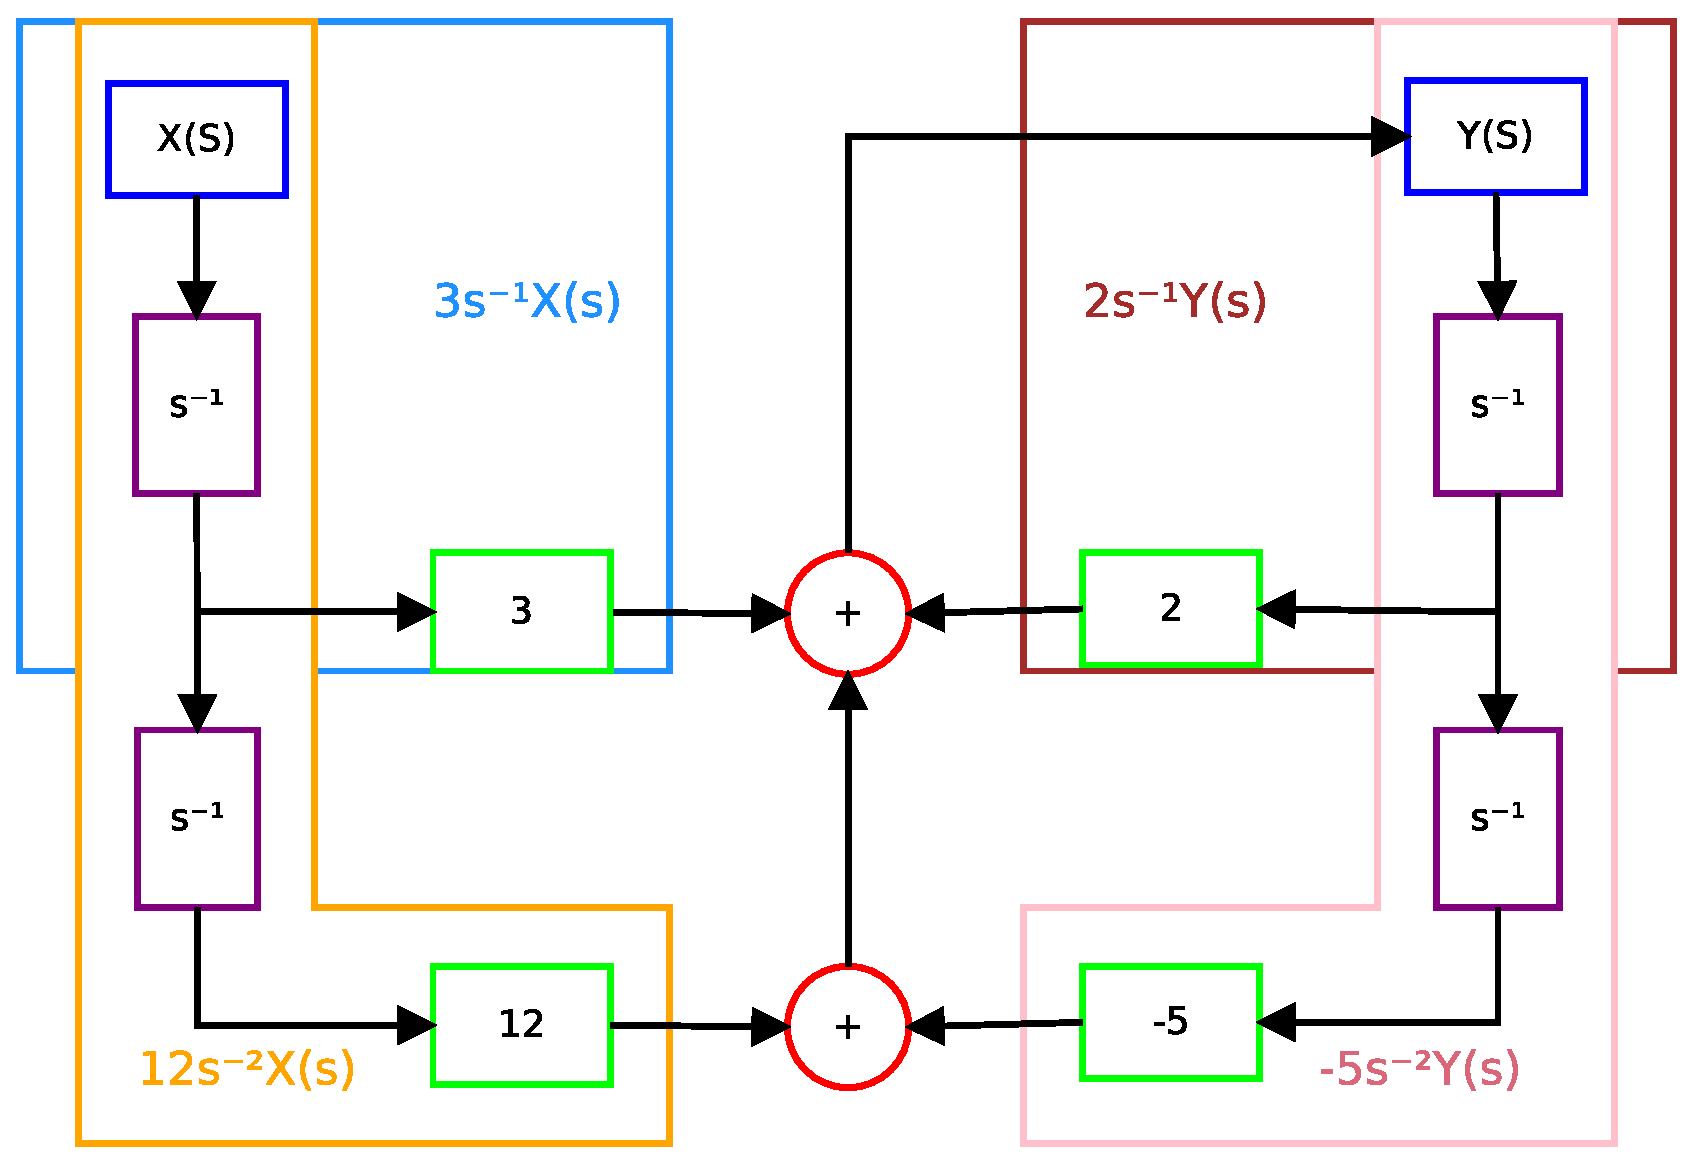
\includegraphics[width=1\linewidth]{./Ejercicio6/Diagrama1_parte4}
          \end{center}
        \end{subfigure}
        \caption{Análisis del diagrama de bloques}
      \end{center}
    \end{figure}
    \begin{figure}[H]
      \begin{center}
        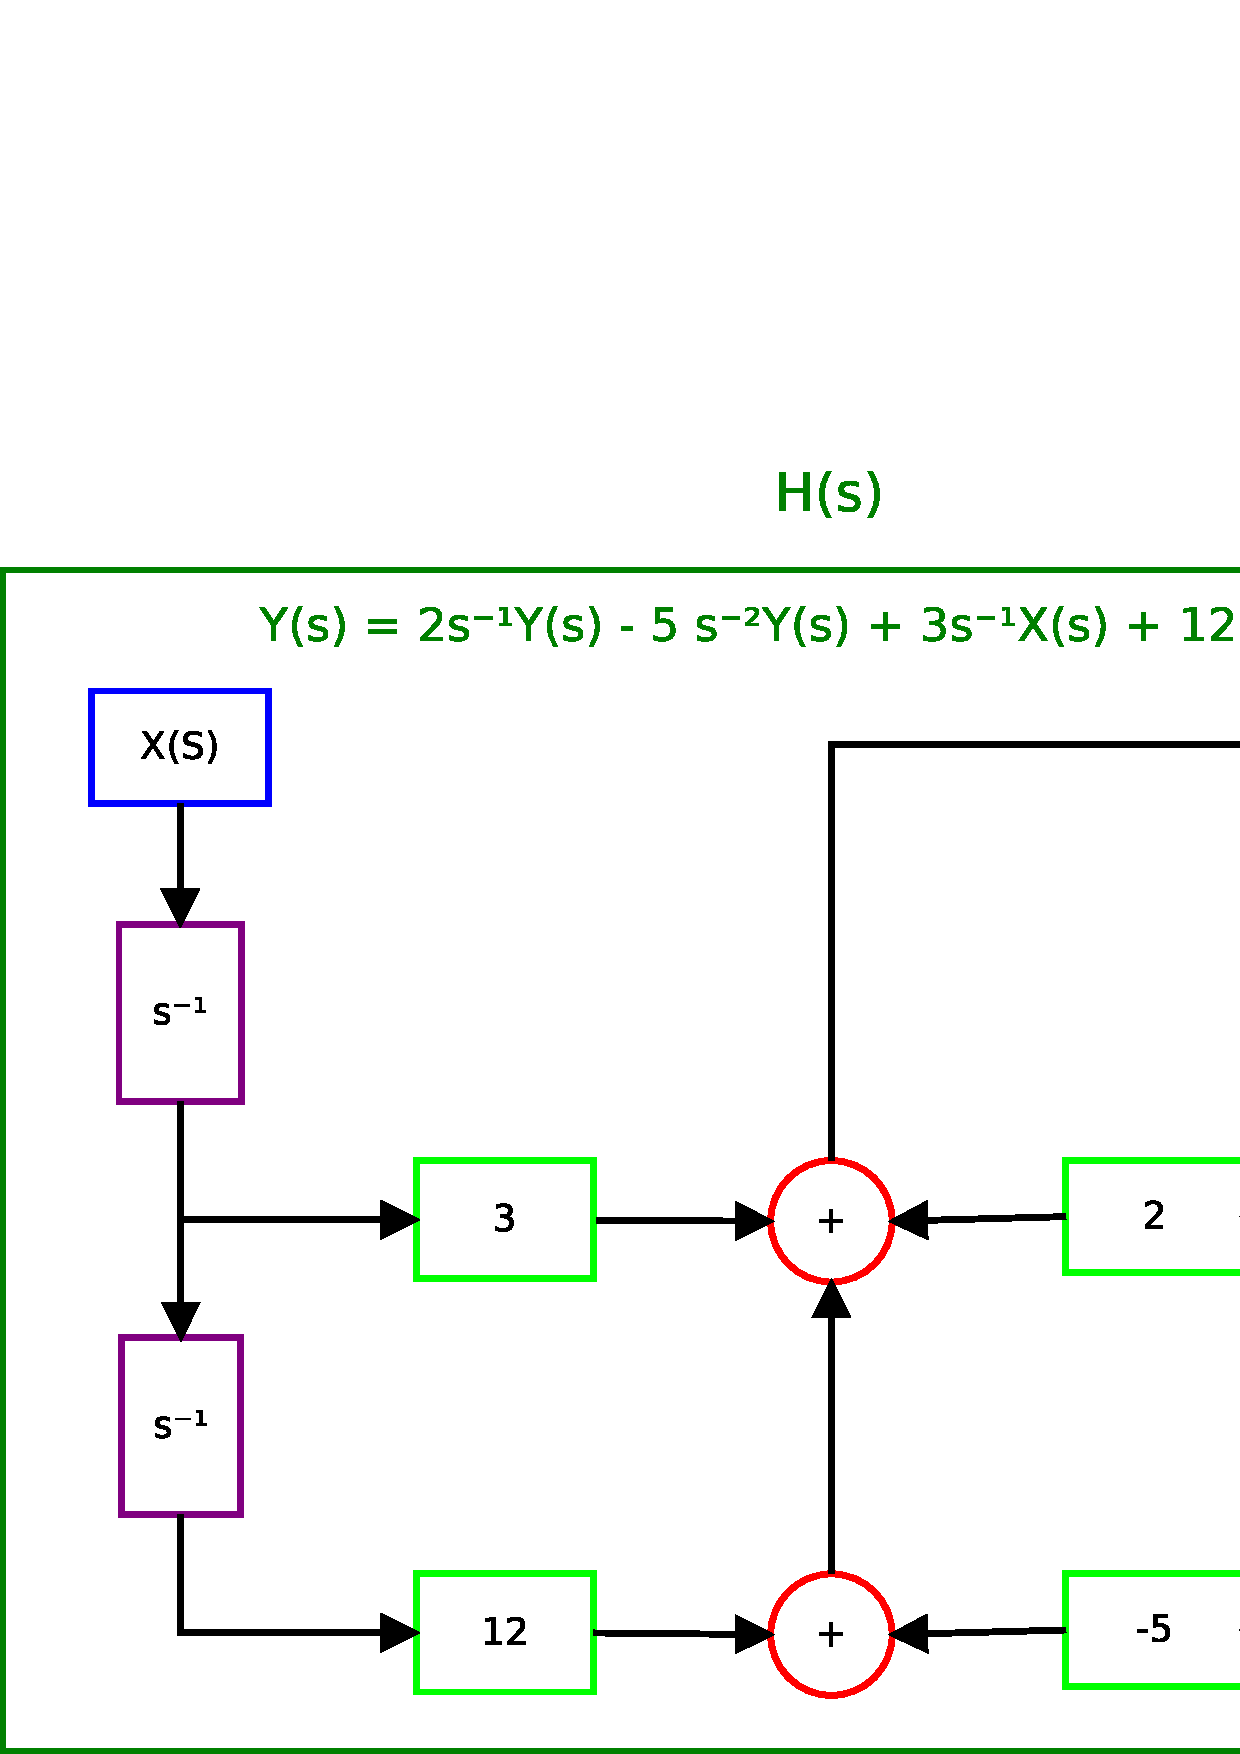
\includegraphics[width=0.6\textwidth]{./Ejercicio6/Diagrama1_parte5}
        \caption{Modelo del sistema en el dominio de s}
      \end{center}
    \end{figure}
    Antitransformando la expresión
    \[\begin{split}
      s^2 \left( -2\frac{Y(s)}{s^2} + 5\frac{Y(s)}{s} + Y(s) = 12\frac{X(s)}{s^2} + 3\frac{X(s)}{s} \right)\\
      \mathcal{L} \left\{ -2Y(s) + 5sY(s) + s^2Y(s) = 12X(s) + 3sX(s) \right\}\\
      \frac{d^2y(t)}{dt^2} + 5\frac{dy(t)}{dt} -2y(t) = 12x(t) + 3\frac{d^x(t)}{dt} 
    \end{split}\]

\end{document}
